% Options for packages loaded elsewhere
\PassOptionsToPackage{unicode}{hyperref}
\PassOptionsToPackage{hyphens}{url}
\PassOptionsToPackage{dvipsnames,svgnames,x11names}{xcolor}
%
\documentclass[
  letterpaper,
  DIV=11,
  numbers=noendperiod]{scrreprt}

\usepackage{amsmath,amssymb}
\usepackage{iftex}
\ifPDFTeX
  \usepackage[T1]{fontenc}
  \usepackage[utf8]{inputenc}
  \usepackage{textcomp} % provide euro and other symbols
\else % if luatex or xetex
  \usepackage{unicode-math}
  \defaultfontfeatures{Scale=MatchLowercase}
  \defaultfontfeatures[\rmfamily]{Ligatures=TeX,Scale=1}
\fi
\usepackage{lmodern}
\ifPDFTeX\else  
    % xetex/luatex font selection
\fi
% Use upquote if available, for straight quotes in verbatim environments
\IfFileExists{upquote.sty}{\usepackage{upquote}}{}
\IfFileExists{microtype.sty}{% use microtype if available
  \usepackage[]{microtype}
  \UseMicrotypeSet[protrusion]{basicmath} % disable protrusion for tt fonts
}{}
\makeatletter
\@ifundefined{KOMAClassName}{% if non-KOMA class
  \IfFileExists{parskip.sty}{%
    \usepackage{parskip}
  }{% else
    \setlength{\parindent}{0pt}
    \setlength{\parskip}{6pt plus 2pt minus 1pt}}
}{% if KOMA class
  \KOMAoptions{parskip=half}}
\makeatother
\usepackage{xcolor}
\setlength{\emergencystretch}{3em} % prevent overfull lines
\setcounter{secnumdepth}{5}
% Make \paragraph and \subparagraph free-standing
\ifx\paragraph\undefined\else
  \let\oldparagraph\paragraph
  \renewcommand{\paragraph}[1]{\oldparagraph{#1}\mbox{}}
\fi
\ifx\subparagraph\undefined\else
  \let\oldsubparagraph\subparagraph
  \renewcommand{\subparagraph}[1]{\oldsubparagraph{#1}\mbox{}}
\fi

\usepackage{color}
\usepackage{fancyvrb}
\newcommand{\VerbBar}{|}
\newcommand{\VERB}{\Verb[commandchars=\\\{\}]}
\DefineVerbatimEnvironment{Highlighting}{Verbatim}{commandchars=\\\{\}}
% Add ',fontsize=\small' for more characters per line
\usepackage{framed}
\definecolor{shadecolor}{RGB}{241,243,245}
\newenvironment{Shaded}{\begin{snugshade}}{\end{snugshade}}
\newcommand{\AlertTok}[1]{\textcolor[rgb]{0.68,0.00,0.00}{#1}}
\newcommand{\AnnotationTok}[1]{\textcolor[rgb]{0.37,0.37,0.37}{#1}}
\newcommand{\AttributeTok}[1]{\textcolor[rgb]{0.40,0.45,0.13}{#1}}
\newcommand{\BaseNTok}[1]{\textcolor[rgb]{0.68,0.00,0.00}{#1}}
\newcommand{\BuiltInTok}[1]{\textcolor[rgb]{0.00,0.23,0.31}{#1}}
\newcommand{\CharTok}[1]{\textcolor[rgb]{0.13,0.47,0.30}{#1}}
\newcommand{\CommentTok}[1]{\textcolor[rgb]{0.37,0.37,0.37}{#1}}
\newcommand{\CommentVarTok}[1]{\textcolor[rgb]{0.37,0.37,0.37}{\textit{#1}}}
\newcommand{\ConstantTok}[1]{\textcolor[rgb]{0.56,0.35,0.01}{#1}}
\newcommand{\ControlFlowTok}[1]{\textcolor[rgb]{0.00,0.23,0.31}{#1}}
\newcommand{\DataTypeTok}[1]{\textcolor[rgb]{0.68,0.00,0.00}{#1}}
\newcommand{\DecValTok}[1]{\textcolor[rgb]{0.68,0.00,0.00}{#1}}
\newcommand{\DocumentationTok}[1]{\textcolor[rgb]{0.37,0.37,0.37}{\textit{#1}}}
\newcommand{\ErrorTok}[1]{\textcolor[rgb]{0.68,0.00,0.00}{#1}}
\newcommand{\ExtensionTok}[1]{\textcolor[rgb]{0.00,0.23,0.31}{#1}}
\newcommand{\FloatTok}[1]{\textcolor[rgb]{0.68,0.00,0.00}{#1}}
\newcommand{\FunctionTok}[1]{\textcolor[rgb]{0.28,0.35,0.67}{#1}}
\newcommand{\ImportTok}[1]{\textcolor[rgb]{0.00,0.46,0.62}{#1}}
\newcommand{\InformationTok}[1]{\textcolor[rgb]{0.37,0.37,0.37}{#1}}
\newcommand{\KeywordTok}[1]{\textcolor[rgb]{0.00,0.23,0.31}{#1}}
\newcommand{\NormalTok}[1]{\textcolor[rgb]{0.00,0.23,0.31}{#1}}
\newcommand{\OperatorTok}[1]{\textcolor[rgb]{0.37,0.37,0.37}{#1}}
\newcommand{\OtherTok}[1]{\textcolor[rgb]{0.00,0.23,0.31}{#1}}
\newcommand{\PreprocessorTok}[1]{\textcolor[rgb]{0.68,0.00,0.00}{#1}}
\newcommand{\RegionMarkerTok}[1]{\textcolor[rgb]{0.00,0.23,0.31}{#1}}
\newcommand{\SpecialCharTok}[1]{\textcolor[rgb]{0.37,0.37,0.37}{#1}}
\newcommand{\SpecialStringTok}[1]{\textcolor[rgb]{0.13,0.47,0.30}{#1}}
\newcommand{\StringTok}[1]{\textcolor[rgb]{0.13,0.47,0.30}{#1}}
\newcommand{\VariableTok}[1]{\textcolor[rgb]{0.07,0.07,0.07}{#1}}
\newcommand{\VerbatimStringTok}[1]{\textcolor[rgb]{0.13,0.47,0.30}{#1}}
\newcommand{\WarningTok}[1]{\textcolor[rgb]{0.37,0.37,0.37}{\textit{#1}}}

\providecommand{\tightlist}{%
  \setlength{\itemsep}{0pt}\setlength{\parskip}{0pt}}\usepackage{longtable,booktabs,array}
\usepackage{calc} % for calculating minipage widths
% Correct order of tables after \paragraph or \subparagraph
\usepackage{etoolbox}
\makeatletter
\patchcmd\longtable{\par}{\if@noskipsec\mbox{}\fi\par}{}{}
\makeatother
% Allow footnotes in longtable head/foot
\IfFileExists{footnotehyper.sty}{\usepackage{footnotehyper}}{\usepackage{footnote}}
\makesavenoteenv{longtable}
\usepackage{graphicx}
\makeatletter
\def\maxwidth{\ifdim\Gin@nat@width>\linewidth\linewidth\else\Gin@nat@width\fi}
\def\maxheight{\ifdim\Gin@nat@height>\textheight\textheight\else\Gin@nat@height\fi}
\makeatother
% Scale images if necessary, so that they will not overflow the page
% margins by default, and it is still possible to overwrite the defaults
% using explicit options in \includegraphics[width, height, ...]{}
\setkeys{Gin}{width=\maxwidth,height=\maxheight,keepaspectratio}
% Set default figure placement to htbp
\makeatletter
\def\fps@figure{htbp}
\makeatother

\KOMAoption{captions}{tableheading}
\makeatletter
\makeatother
\makeatletter
\@ifpackageloaded{bookmark}{}{\usepackage{bookmark}}
\makeatother
\makeatletter
\@ifpackageloaded{caption}{}{\usepackage{caption}}
\AtBeginDocument{%
\ifdefined\contentsname
  \renewcommand*\contentsname{Table of contents}
\else
  \newcommand\contentsname{Table of contents}
\fi
\ifdefined\listfigurename
  \renewcommand*\listfigurename{List of Figures}
\else
  \newcommand\listfigurename{List of Figures}
\fi
\ifdefined\listtablename
  \renewcommand*\listtablename{List of Tables}
\else
  \newcommand\listtablename{List of Tables}
\fi
\ifdefined\figurename
  \renewcommand*\figurename{Figure}
\else
  \newcommand\figurename{Figure}
\fi
\ifdefined\tablename
  \renewcommand*\tablename{Table}
\else
  \newcommand\tablename{Table}
\fi
}
\@ifpackageloaded{float}{}{\usepackage{float}}
\floatstyle{ruled}
\@ifundefined{c@chapter}{\newfloat{codelisting}{h}{lop}}{\newfloat{codelisting}{h}{lop}[chapter]}
\floatname{codelisting}{Listing}
\newcommand*\listoflistings{\listof{codelisting}{List of Listings}}
\makeatother
\makeatletter
\@ifpackageloaded{caption}{}{\usepackage{caption}}
\@ifpackageloaded{subcaption}{}{\usepackage{subcaption}}
\makeatother
\makeatletter
\@ifpackageloaded{tcolorbox}{}{\usepackage[skins,breakable]{tcolorbox}}
\makeatother
\makeatletter
\@ifundefined{shadecolor}{\definecolor{shadecolor}{rgb}{.97, .97, .97}}
\makeatother
\makeatletter
\makeatother
\makeatletter
\makeatother
\ifLuaTeX
  \usepackage{selnolig}  % disable illegal ligatures
\fi
\IfFileExists{bookmark.sty}{\usepackage{bookmark}}{\usepackage{hyperref}}
\IfFileExists{xurl.sty}{\usepackage{xurl}}{} % add URL line breaks if available
\urlstyle{same} % disable monospaced font for URLs
\hypersetup{
  pdftitle={Quantitative Methods 2},
  pdfauthor={Ollie Ballinger},
  colorlinks=true,
  linkcolor={blue},
  filecolor={Maroon},
  citecolor={Blue},
  urlcolor={Blue},
  pdfcreator={LaTeX via pandoc}}

\title{Quantitative Methods 2}
\author{Ollie Ballinger}
\date{2023-10-10}

\begin{document}
\maketitle
\ifdefined\Shaded\renewenvironment{Shaded}{\begin{tcolorbox}[interior hidden, borderline west={3pt}{0pt}{shadecolor}, boxrule=0pt, frame hidden, enhanced, sharp corners, breakable]}{\end{tcolorbox}}\fi

\renewcommand*\contentsname{Table of contents}
{
\hypersetup{linkcolor=}
\setcounter{tocdepth}{2}
\tableofcontents
}
\bookmarksetup{startatroot}

\hypertarget{welcome}{%
\chapter*{Welcome}\label{welcome}}
\addcontentsline{toc}{chapter}{Welcome}

\markboth{Welcome}{Welcome}

\hypertarget{welcome-to-basc0005---quantitative-methods-data-science-and-visualisation}{%
\section*{Welcome to BASC0005 - Quantitative Methods: Data Science and
Visualisation}\label{welcome-to-basc0005---quantitative-methods-data-science-and-visualisation}}
\addcontentsline{toc}{section}{Welcome to BASC0005 - Quantitative
Methods: Data Science and Visualisation}

\markright{Welcome to BASC0005 - Quantitative Methods: Data Science and
Visualisation}

This course teaches quantitative skills, with an emphasis on the context
and use of data. Students learn to focus on datasets which will allow
them to explore questions in society -- in arts, humanities, sports,
criminal justice, economics, inequality, or policy. Students are
expected to work with Python to carry out data manipulation (cleaning
and segmentation), analysis (for example, deriving descriptive
statistics) and visualisation (graphing, mapping and other forms of
visualisation). They will engage with literatures around a topic and
connect their datasets and analyses to explore and decide wider
arguments, and link their results to these contextual considerations.
Below is an outline of the course:

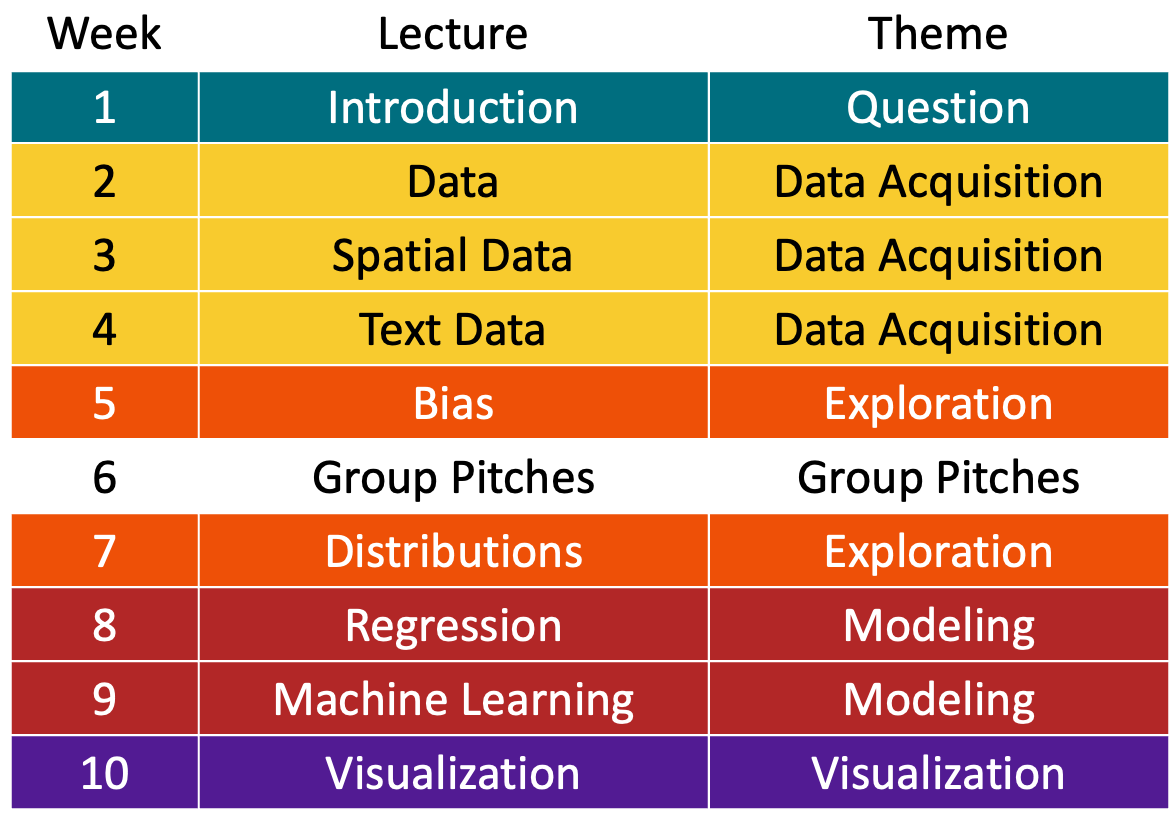
\includegraphics{outline.png}

\bookmarksetup{startatroot}

\hypertarget{python-recap}{%
\chapter{Python Recap}\label{python-recap}}

\hypertarget{workshop-1-open-in-colab}{%
\section[\emph{Workshop 1} ]{\texorpdfstring{\emph{Workshop 1}
\href{https://colab.research.google.com/github/oballinger/QM2/blob/main/notebooks/W01.\%20Python\%20Recap.ipynb}{\protect
\includegraphics{index_files/mediabag/colab-badge.png}}}{Workshop 1 Open In Colab}}\label{workshop-1-open-in-colab}}

\hypertarget{registering-a-github-account}{%
\section{Registering a GitHub
account}\label{registering-a-github-account}}

Before we get started, we need to set a few things up. GitHub is a
platform for software development and version control using Git,
allowing developers to store and manage their code. Think of it as
google docs but for code-- it will be very useful for collaborating on
your group projects later in the term, and in your future as a data
analyst.

\begin{enumerate}
\def\labelenumi{\arabic{enumi}.}
\tightlist
\item
  Use \href{https://github.com/join}{this link} to register for a GitHub
  account if you don't already have one.
\item
  Once that's done, \href{https://github.com/new}{create a new github
  repository} called ``QM2''.
\item
  In this notebook, click ``File'' and then ``Save a copy in GitHub''.
\end{enumerate}

Voila! You now have a version of this notebook saved to your own GitHub
account. \emph{You will need to do step 3 for all the workshops!} Now,
on to python.

\hypertarget{using-python}{%
\section{Using Python}\label{using-python}}

In this course, we'll make extensive use of \emph{Python}, a programming
language used widely in scientific computing and on the web. We will be
using Python as a way to manipulate, plot and analyse data. This isn't a
course about learning Python, it's about working with data - but we'll
learning a little bit of programming along the way.

By now, you should have done the prerequisites for the module, and
understand a bit about how Python is structured, what different commands
do, and so on - this is a bit of a refresher to remind you of what we
need at the beginning of term.

The particular flavour of Python we're using is \emph{iPython}, which,
as we've seen, allows us to combine text, code, images, equations and
figures in a \emph{Notebook}. This is a \emph{cell}, written in
\emph{markdown} - a way of writing nice text. Contrast this with
\emph{code} cell, which executes a bit of Python:

\begin{Shaded}
\begin{Highlighting}[]
\BuiltInTok{print}\NormalTok{(}\DecValTok{2}\OperatorTok{+}\DecValTok{2}\NormalTok{)}
\end{Highlighting}
\end{Shaded}

\begin{verbatim}
4
\end{verbatim}

The Notebook format allows you to engage in what Don Knuth describes as
\href{http://en.wikipedia.org/wiki/Literate_programming}{Literate
Programming}:

\begin{quote}
{[}\ldots{]} Instead of writing code containing documentation, the
literate programmer writes documentation containing code. No longer does
the English commentary injected into a program have to be hidden in
comment delimiters at the top of the file, or under procedure headings,
or at the end of lines. Instead, it is wrenched into the daylight and
made the main focus. The ``program'' then becomes primarily a document
directed at humans, with the code being herded between ``code
delimiters'' from where it can be extracted and shuffled out sideways to
the language system by literate programming tools.
\href{http://www.literateprogramming.com/lpquotes.html}{Ross Williams}
\end{quote}

\hypertarget{libraries}{%
\section{Libraries}\label{libraries}}

We will work with a number of \emph{libraries}, which provide additional
functions and techniques to help us to carry out our tasks.

These include:

\emph{Pandas:} we'll use this a lot to slice and dice data

\emph{matplotlib}: this is our basic graphing software, and we'll also
use it for mapping

\emph{nltk}: The Natural Language Tool Kit will help us work with text

We aren't doing all this to learn to program. We could spend a whole
term learning how to use Python and never look at any data, maps,
graphs, or visualisations. But we do need to understand a few basics to
use Python for working with data. So let's revisit a few concepts that
you should have covered in your prerequisites.

\hypertarget{variables}{%
\section{Variables}\label{variables}}

Python can broadly be divided in verbs and nouns: things which \emph{do}
things, and things which \emph{are} things. In Python, the verbs can be
\emph{commands}, \emph{functions}, or \emph{methods}. We won't worry too
much about the distinction here - suffice it to say, they are the parts
of code which manipulate data, calculate values, or show things on the
screen.

The simplest proper noun object in Python is the \emph{variable}.
Variables are given names and store information. This can be, for
example, numeric, text, or boolean (true/false). These are all
statements setting up variables:

n = 1

t = ``hi''

b = True

Now let's try this in code:

\begin{Shaded}
\begin{Highlighting}[]
\NormalTok{n }\OperatorTok{=} \DecValTok{1}

\NormalTok{t }\OperatorTok{=} \StringTok{"hi"}

\NormalTok{b }\OperatorTok{=} \VariableTok{True}
\end{Highlighting}
\end{Shaded}

Note that each command is on a new line; other than that, the
\emph{syntax} of Python should be fairly clear. We're setting these
variables equal to the letters and numbers and phrases and booleans.
\textbf{What's a boolean?}

The value of this is we now have values tied to these variables - so
every time we want to use it, we can refer to the variable:

\begin{Shaded}
\begin{Highlighting}[]
\NormalTok{n}
\end{Highlighting}
\end{Shaded}

\begin{verbatim}
1
\end{verbatim}

\begin{Shaded}
\begin{Highlighting}[]
\NormalTok{t}
\end{Highlighting}
\end{Shaded}

\begin{verbatim}
'hi'
\end{verbatim}

\begin{Shaded}
\begin{Highlighting}[]
\NormalTok{b}
\end{Highlighting}
\end{Shaded}

\begin{verbatim}
True
\end{verbatim}

Because we've defined these variables in the early part of the notebook,
we can use them later on.

\emph{\textbf{Advanced}: where do \textbf{classes} fit into this
noun/verb picture of variables and commands?}

\hypertarget{where-is-my-data}{%
\section{Where is my data?}\label{where-is-my-data}}

When we work in excel and text editors, we're used to seeing the data
onscreen - and if we manipulate the data in some way (averaging or
summing up), we see both the inputs and outputs on screen. The big
difference in working with Python is that we don't see our variables all
of the time, or the effect we're having on them. They're there in the
background, but it's usually worth checking in on them from time to
time, to see whether our processes are doing what we think they're
doing.

This is pretty easy to do - we can just type the variable name, or
``print(\emph{variable name})'':

\begin{Shaded}
\begin{Highlighting}[]
\NormalTok{n }\OperatorTok{=}\NormalTok{ n}\OperatorTok{+}\DecValTok{1}
\BuiltInTok{print}\NormalTok{(n)}
\BuiltInTok{print}\NormalTok{(t)}
\BuiltInTok{print}\NormalTok{(b)}
\end{Highlighting}
\end{Shaded}

\begin{verbatim}
2
hi
True
\end{verbatim}

\hypertarget{flow}{%
\section{Flow}\label{flow}}

Python, in common with all programming languages, executes commands in a
sequence - we might refer to this as the ``ineluctable march of the
machines'', but it's more common referred to as the \emph{flow} of the
code (we'll use the word ``code'' a lot - it just means commands written
in the programming language). In most cases, code just executes in the
order it's written. This is true within each \emph{cell} (each block of
text in the notebook), and it's true when we execute the cells in order;
that's why we can refer back to the variables we defined earlier:

\begin{Shaded}
\begin{Highlighting}[]
\BuiltInTok{print}\NormalTok{(n)}
\end{Highlighting}
\end{Shaded}

\begin{verbatim}
2
\end{verbatim}

If we make a change to one of these variables, say n:

\begin{Shaded}
\begin{Highlighting}[]
\NormalTok{n }\OperatorTok{=} \DecValTok{3}
\end{Highlighting}
\end{Shaded}

and execute the above ``print n'' command, you'll see that it has
changed n to 3. So if we go out of order, the obvious flow of the code
is confused. For this reason, try to write your code so it executes in
order, one cell at a time. At least for the moment, this will make it
easier to follow the logic of what you're doing to data.

\emph{Advanced}: what happens to this flow when you write
\emph{functions} to automate common tasks?

\textbf{\emph{Exercise - Setting up variables}}:

\begin{enumerate}
\def\labelenumi{\arabic{enumi}.}
\item
  Create a new cell.
\item
  Create the variables ``name'', and assign your name to it.
\item
  Create a variable ``Python'' and assign a score out of 10 to how much
  you like Python.
\item
  Create a variable ``prior'' and if you've used Python before, assign
  True; otherwise assign False to the variable
\item
  Print these out to the screen
\end{enumerate}

\hypertarget{downloading-data}{%
\section{Downloading Data}\label{downloading-data}}

Lets fetch the data we will be using for this session. There are two
ways in which you can upload data to the Colab notebook. You can use the
following code to upload a CSV or similar data file.

\begin{Shaded}
\begin{Highlighting}[]
\ImportTok{from}\NormalTok{ google.colab }\ImportTok{import}\NormalTok{ files}
\NormalTok{uploaded }\OperatorTok{=}\NormalTok{ files.upload()}
\end{Highlighting}
\end{Shaded}

Or you can use the following cell to fetch the data directly from the
QM2 server.

Let's create a folder that we can store all our data for this session

\begin{Shaded}
\begin{Highlighting}[]
\OperatorTok{!}\NormalTok{mkdir data}
\end{Highlighting}
\end{Shaded}

\begin{Shaded}
\begin{Highlighting}[]
\OperatorTok{!}\NormalTok{mkdir .}\OperatorTok{/}\NormalTok{data}\OperatorTok{/}\NormalTok{wk1}
\OperatorTok{!}\NormalTok{curl https:}\OperatorTok{//}\NormalTok{s3.eu}\OperatorTok{{-}}\NormalTok{west}\OperatorTok{{-}}\FloatTok{2.}\ErrorTok{amazonaws}\NormalTok{.com}\OperatorTok{/}\NormalTok{qm2}\OperatorTok{/}\NormalTok{wk1}\OperatorTok{/}\NormalTok{data.csv }\OperatorTok{{-}}\NormalTok{o .}\OperatorTok{/}\NormalTok{data}\OperatorTok{/}\NormalTok{wk1}\OperatorTok{/}\NormalTok{data.csv}
\OperatorTok{!}\NormalTok{curl https:}\OperatorTok{//}\NormalTok{s3.eu}\OperatorTok{{-}}\NormalTok{west}\OperatorTok{{-}}\FloatTok{2.}\ErrorTok{amazonaws}\NormalTok{.com}\OperatorTok{/}\NormalTok{qm2}\OperatorTok{/}\NormalTok{wk1}\OperatorTok{/}\NormalTok{sample\_group.csv }\OperatorTok{{-}}\NormalTok{o .}\OperatorTok{/}\NormalTok{data}\OperatorTok{/}\NormalTok{wk1}\OperatorTok{/}\NormalTok{sample\_group.csv}
\end{Highlighting}
\end{Shaded}

\begin{verbatim}
  % Total    % Received % Xferd  Average Speed   Time    Time     Time  Current
                                 Dload  Upload   Total   Spent    Left  Speed
100   203  100   203    0     0   2872      0 --:--:-- --:--:-- --:--:--  3029
  % Total    % Received % Xferd  Average Speed   Time    Time     Time  Current
                                 Dload  Upload   Total   Spent    Left  Speed
100   297  100   297    0     0   1844      0 --:--:-- --:--:-- --:--:--  1879
\end{verbatim}

\hypertarget{storing-and-importing-data}{%
\section{Storing and importing data}\label{storing-and-importing-data}}

Typically, data we look at won't be just one number, or one bit of text.
Python has a lot of different ways of dealing with a bunch of numbers:
for example, a list of values is called a \textbf{list}:

\begin{Shaded}
\begin{Highlighting}[]
\NormalTok{listy }\OperatorTok{=}\NormalTok{ [}\DecValTok{1}\NormalTok{,}\DecValTok{2}\NormalTok{,}\DecValTok{3}\NormalTok{,}\DecValTok{6}\NormalTok{,}\DecValTok{9}\NormalTok{]}
\BuiltInTok{print}\NormalTok{(listy)}
\end{Highlighting}
\end{Shaded}

\begin{verbatim}
[1, 2, 3, 6, 9]
\end{verbatim}

A set of values \emph{linked} to an index (or key) is called a
\textbf{dictionary}; for example:

\begin{Shaded}
\begin{Highlighting}[]
\NormalTok{dicty }\OperatorTok{=}\NormalTok{ \{}\StringTok{\textquotesingle{}Bob\textquotesingle{}}\NormalTok{: }\FloatTok{1.2}\NormalTok{, }\StringTok{\textquotesingle{}Mike\textquotesingle{}}\NormalTok{: }\FloatTok{1.2}\NormalTok{, }\StringTok{\textquotesingle{}Coop\textquotesingle{}}\NormalTok{: }\FloatTok{1.1}\NormalTok{, }\StringTok{\textquotesingle{}Maddy\textquotesingle{}}\NormalTok{: }\FloatTok{1.3}\NormalTok{, }\StringTok{\textquotesingle{}Giant\textquotesingle{}}\NormalTok{: }\FloatTok{2.1}\NormalTok{\}}
\BuiltInTok{print}\NormalTok{(dicty)}
\end{Highlighting}
\end{Shaded}

\begin{verbatim}
{'Bob': 1.2, 'Mike': 1.2, 'Coop': 1.1, 'Maddy': 1.3, 'Giant': 2.1}
\end{verbatim}

Notice that the list uses square brackets with values separated by
commas, and the dict uses curly brackets with pairs separated by commas,
and colons (:) to link a \emph{key} (index or address) with a value.

(You might notice that they haven't printed out in the order you entered
them)

*\textbf{Advanced}: Print out 1) The third element of \textbf{listy},
and 2) The element of \textbf{dicty} relating to Giant

We'll discuss different ways of organising data again soon, but for now
we'll look at \emph{dataframes} - the way our data-friendly
\emph{library} \textbf{Pandas} works with data. We'll be using Pandas a
lot this term, so it's good to get started with it early.

Let's start by importing pandas. We'll also import another library, but
we're not going to worry about that too much at the moment.

If you see a warning about `Building Font Cache' don't worry - this is
normal.

\begin{Shaded}
\begin{Highlighting}[]
\ImportTok{import}\NormalTok{ pandas}

\ImportTok{import}\NormalTok{ matplotlib}
\OperatorTok{\%}\NormalTok{matplotlib inline}
\end{Highlighting}
\end{Shaded}

Let's import a simple dataset and show it in pandas. We'll use a
pre-prepared ``.csv'' file, which needs to be in the same folder as our
code.

\begin{Shaded}
\begin{Highlighting}[]
\NormalTok{data }\OperatorTok{=}\NormalTok{ pandas.read\_csv(}\StringTok{\textquotesingle{}./data/wk1/data.csv\textquotesingle{}}\NormalTok{)}
\NormalTok{data.head()}
\end{Highlighting}
\end{Shaded}

\begin{longtable}[]{@{}llllll@{}}
\toprule\noalign{}
& Name & First Appearance & Approx height & Gender & Law Enforcement \\
\midrule\noalign{}
\endhead
\bottomrule\noalign{}
\endlastfoot
0 & Bob & 1.2 & 6.0 & Male & False \\
1 & Mike & 1.2 & 5.5 & Male & False \\
2 & Coop & 1.1 & 6.0 & Male & True \\
3 & Maddy & 1.3 & 5.5 & Female & False \\
4 & Giant & 2.1 & 7.5 & Male & False \\
\end{longtable}

What we've done here is read in a .csv file into a dataframe, the object
pandas uses to work with data, and one that has lots of methods for
slicing and dicing data, as we will see over the coming weeks. The
head() command tells iPython to show the first few columns/rows of the
data, so we can start to get a sense of what the data looks like and
what sort of type of objects is represents.

A common first step for exploring our data is to sort it. In Pandas,
this can be done easily with the \texttt{sort\_values()} function. We
can specify which column to sort the data by, and whether we want to
sort in ascending or descending order, using the optional arguments
\texttt{by} and \texttt{ascending}, respectively. In the example below,
we're sorting in \emph{descending} order of height:

\begin{Shaded}
\begin{Highlighting}[]
\NormalTok{data.sort\_values(by}\OperatorTok{=}\StringTok{\textquotesingle{}Approx height\textquotesingle{}}\NormalTok{, ascending}\OperatorTok{=}\VariableTok{False}\NormalTok{).head()}
\end{Highlighting}
\end{Shaded}

\begin{longtable}[]{@{}llllll@{}}
\toprule\noalign{}
& Name & First Appearance & Approx height & Gender & Law Enforcement \\
\midrule\noalign{}
\endhead
\bottomrule\noalign{}
\endlastfoot
4 & Giant & 2.1 & 7.5 & Male & False \\
0 & Bob & 1.2 & 6.0 & Male & False \\
2 & Coop & 1.1 & 6.0 & Male & True \\
1 & Mike & 1.2 & 5.5 & Male & False \\
3 & Maddy & 1.3 & 5.5 & Female & False \\
\end{longtable}

\bookmarksetup{startatroot}

\hypertarget{supplementary-kaggle-exercises}{%
\chapter{Supplementary: Kaggle
exercises}\label{supplementary-kaggle-exercises}}

If you've gotten this far, congratulations! To further hone your skills,
try working your way through the five
\href{https://www.kaggle.com/learn/intro-to-programming}{intro to
programming notebooks on Kaggle}. These cover a range of skills that
we'll be using throughout the term. Kaggle is a very useful resource for
learning data science, so making an account may not be a bad idea!

\bookmarksetup{startatroot}

\hypertarget{assessed-question}{%
\chapter{Assessed Question}\label{assessed-question}}

The URL below contains a dataset of the most streamed songs on spotify
in 2023: https://storage.googleapis.com/qm2/wk1/spotify-2023.csv

\begin{enumerate}
\def\labelenumi{\arabic{enumi}.}
\tightlist
\item
  Download the dataset and save it in the \texttt{./data/wk1/}
  directory.
\item
  Load the dataset as a pandas dataframe, and inspect it. Two of the
  column names have accidentally been swapped around. Use common sense
  to figure out which ones these are before proceeding with your
  analysis.
\item
  Filter the dataset to only contain songs in the key of C sharp.
\item
  Sort the dataframe in descending order of streams.
\end{enumerate}

QUESTION: which artist has the song with the highest number of streams?

\begin{Shaded}
\begin{Highlighting}[]
\CommentTok{\# use this code cell to answer the question}
\end{Highlighting}
\end{Shaded}

\bookmarksetup{startatroot}

\hypertarget{intro-to-pandas}{%
\chapter{Intro to Pandas}\label{intro-to-pandas}}

\hypertarget{workshop-2-open-in-colab}{%
\section[\emph{Workshop 2} ]{\texorpdfstring{\emph{Workshop 2}
\href{https://colab.research.google.com/github/oballinger/QM2/blob/main/notebooks/W02.\%20Pandas.ipynb}{\protect
\includegraphics{notebooks/../colab-badge.png}}}{Workshop 2 Open In Colab}}\label{workshop-2-open-in-colab}}

In this workshop, our aim is to get used to working with more complex
data that we've imported from external files. We'll start to graph it,
and to slice and dice it, to select the bits we're interested in.

We will work with \emph{pandas} to manipulate the data, and to derive
measures and graphs that tell us a bit more than what the source data
files tell us.

\hypertarget{aims}{%
\subsection{Aims}\label{aims}}

\begin{itemize}
\tightlist
\item
  Learn to import data to python using pandas
\item
  Learn how access specific rows, columns and cells
\item
  Plot the data
\item
  Tidy up graphs to include axes
\end{itemize}

\hypertarget{introduction}{%
\section{Introduction}\label{introduction}}

We are going to work with some UK income data. The income data is
packaged as a .csv file. The Pandas package knows how to handle this and
put the data in a DataFrame, as we've seen. Let's examine the data and
start to see what we can say about it. First of all, we have to find
data - I'm interested in looking in data with a wide spread, so I looked
for data on income in the UK.

This data is collected by the Office for National Statistics(ONS) :
http://www.ons.gov.uk/ons/datasets-and-tables/index.html?pageSize=50\&sortBy=none\&sortDirection=none\&newquery=income+percentile
- but the exact data I want to see, income by percentile, is tricky to
find.

I ended up using data from 2011, generated from a study called the
Family Resources Survey and collated and tweaked by an independent
research unit called the Institute of Fiscal Studies (IFS). The
``tweaking'' they do tends to be around the size of the family unit, and
other factors which create economies of scale - hence they
``equivalise'' it. The IFS is quoted in UK Government documents, so we
can have some trust in their impartiality, or at least accuracy - of
course, if we were publishing research about this, that's not really
good enough and we'd want to reproduce, or at least understand and
critique, their methodology rather than just trusting it!

e.g.:

http://www.ifs.org.uk/wheredoyoufitin/about.php

https://en.wikipedia.org/wiki/Equivalisation

\hypertarget{downloading-the-data}{%
\section{Downloading the Data}\label{downloading-the-data}}

Let's grab our income data from our course website and save it into our
data folder. If you've not already created a data folder then do so
using the following command. Don't worry if it generates an error, that
means you've already got a data folder.

\begin{Shaded}
\begin{Highlighting}[]
\OperatorTok{!}\NormalTok{mkdir data}
\end{Highlighting}
\end{Shaded}

\begin{verbatim}
mkdir: data: File exists
\end{verbatim}

\begin{Shaded}
\begin{Highlighting}[]
\OperatorTok{!}\NormalTok{mkdir data}\OperatorTok{/}\NormalTok{wk2}
\OperatorTok{!}\NormalTok{curl https:}\OperatorTok{//}\NormalTok{s3.eu}\OperatorTok{{-}}\NormalTok{west}\OperatorTok{{-}}\FloatTok{2.}\ErrorTok{amazonaws}\NormalTok{.com}\OperatorTok{/}\NormalTok{qm2}\OperatorTok{/}\NormalTok{wk2}\OperatorTok{/}\NormalTok{incomes.csv }\OperatorTok{{-}}\NormalTok{o .}\OperatorTok{/}\NormalTok{data}\OperatorTok{/}\NormalTok{wk2}\OperatorTok{/}\NormalTok{incomes.csv}
\end{Highlighting}
\end{Shaded}

\begin{verbatim}
mkdir: data/wk2: File exists
  % Total    % Received % Xferd  Average Speed   Time    Time     Time  Current
                                 Dload  Upload   Total   Spent    Left  Speed
100 15154  100 15154    0     0   135k      0 --:--:-- --:--:-- --:--:--  143k
\end{verbatim}

\begin{Shaded}
\begin{Highlighting}[]
\ImportTok{import}\NormalTok{ pandas}
\ImportTok{import}\NormalTok{ pylab}
\ImportTok{import}\NormalTok{ matplotlib.pyplot }\ImportTok{as}\NormalTok{ plt}
\CommentTok{\# make the plots a little wider by default}
\OperatorTok{\%}\NormalTok{matplotlib inline}
\NormalTok{plt.style.use(}\StringTok{\textquotesingle{}ggplot\textquotesingle{}}\NormalTok{)}

\NormalTok{pylab.rcParams[}\StringTok{\textquotesingle{}figure.figsize\textquotesingle{}}\NormalTok{] }\OperatorTok{=}\NormalTok{ (}\FloatTok{10.}\NormalTok{, }\FloatTok{8.}\NormalTok{)}
\end{Highlighting}
\end{Shaded}

\begin{Shaded}
\begin{Highlighting}[]
\NormalTok{data\_path }\OperatorTok{=} \StringTok{"./data/wk2/incomes.csv"}

\NormalTok{income }\OperatorTok{=}\NormalTok{  pandas.read\_csv(data\_path, index\_col}\OperatorTok{=}\DecValTok{0}\NormalTok{)}
\NormalTok{income.head()}
\end{Highlighting}
\end{Shaded}

\begin{longtable}[]{@{}llllllllllllllll@{}}
\toprule\noalign{}
& Net equivalised household income in 2010-11, week & Childless couple,
annual income & Couple, two children under 14 & Couple, three children
under 14 & Couple with one child under 14 & Couple with two children
aged 15 to 18 & Couple, two children under 14 plus dependent adult &
Single adult & Lone parent, one child under 14 & Lone parent, two
children under 14 & Lone parent, two children aged 15-18 & ANNOTATIONS &
1979 to 1996-97 & 1996-97 to 2009-10 & 1996-97 to 2010-11 \\
Percentile Point & & & & & & & & & & & & & & & \\
\midrule\noalign{}
\endhead
\bottomrule\noalign{}
\endlastfoot
1 & 33.50 & 1,746.92 & 2,445.69 & 2,795.08 & 2,096.31 & 2,899.89 &
3,022.18 & 1,170.44 & 1,519.82 & 1,869.21 & 2,323.41 & NaN & NaN & NaN &
NaN \\
2 & 98.60 & 5,141.01 & 7,197.41 & 8,225.61 & 6,169.21 & 8,534.07 &
8,893.95 & 3,444.48 & 4,472.68 & 5,500.88 & 6,837.54 & NaN & -0.20\% &
-1.30\% & -0.50\% \\
3 & 128.56 & 6,703.11 & 9,384.36 & 10,724.98 & 8,043.74 & 11,127.17 &
11,596.39 & 4,491.09 & 5,831.71 & 7,172.33 & 8,915.14 & NaN & 0.40\% &
0.10\% & 0.10\% \\
4 & 151.05 & 7,875.75 & 11,026.05 & 12,601.20 & 9,450.90 & 13,073.75 &
13,625.05 & 5,276.75 & 6,851.90 & 8,427.05 & 10,474.75 & NaN & 0.50\% &
0.80\% & 0.60\% \\
5 & 166.32 & 8,671.91 & 12,140.68 & 13,875.06 & 10,406.30 & 14,395.38 &
15,002.41 & 5,810.18 & 7,544.57 & 9,278.95 & 11,533.65 & NaN & 0.70\% &
1.00\% & 0.90\% \\
\end{longtable}

This is a simple dataframe - we see the percentile and an income. Note
that I've told pandas to use the first column (the Percentile) as the
index to make life easier.

The percentile tells us how people on that income rank - so the final
category, 99\% (which is really binned, so 99\%\textless n\(\leq\)
100\%), is telling us how much ``the 1\%'' earn. Let's find out:

\begin{Shaded}
\begin{Highlighting}[]
\NormalTok{income.tail()}
\end{Highlighting}
\end{Shaded}

\begin{longtable}[]{@{}llllllllllllllll@{}}
\toprule\noalign{}
& Net equivalised household income in 2010-11, week & Childless couple,
annual income & Couple, two children under 14 & Couple, three children
under 14 & Couple with one child under 14 & Couple with two children
aged 15 to 18 & Couple, two children under 14 plus dependent adult &
Single adult & Lone parent, one child under 14 & Lone parent, two
children under 14 & Lone parent, two children aged 15-18 & ANNOTATIONS &
1979 to 1996-97 & 1996-97 to 2009-10 & 1996-97 to 2010-11 \\
Percentile Point & & & & & & & & & & & & & & & \\
\midrule\noalign{}
\endhead
\bottomrule\noalign{}
\endlastfoot
95 & 1075.73 & 56,088.56 & 78,523.99 & 89,741.70 & 67,306.27 & 93,107.01
& 97,033.21 & 37,579.34 & 48,797.05 & 60,014.76 & 74,597.79 & NaN &
2.90\% & 2.00\% & 1.30\% \\
96 & 1174.48 & 61,237.18 & 85,732.05 & 97,979.49 & 73,484.61 &
101,653.72 & 105,940.32 & 41,028.91 & 53,276.35 & 65,523.78 & 81,445.45
& NaN & 3.00\% & 2.00\% & 1.40\% \\
97 & 1302.74 & 67,925.07 & 95,095.10 & 108,680.12 & 81,510.09 &
112,755.62 & 117,510.37 & 45,509.80 & 59,094.81 & 72,679.83 & 90,340.35
& NaN & 3.20\% & 2.20\% & 1.60\% \\
98 & 1523.31 & 79,425.23 & 111,195.32 & 127,080.36 & 95,310.27 &
131,845.88 & 137,405.64 & 53,214.90 & 69,099.95 & 84,984.99 & 105,635.55
& NaN & 3.20\% & 2.70\% & 1.70\% \\
99 & 2090.35 & 108,990.74 & 152,587.04 & 174,385.19 & 130,788.89 &
180,924.64 & 188,553.99 & 73,023.80 & 94,821.95 & 116,620.10 &
144,957.69 & NaN & NaN & NaN & NaN \\
\end{longtable}

Well, they we have it - the 1\% earn, on average, about £2000 a week.
How does that compare to people in the 90\% decile? We can access
particular \emph{rows} in a dataframe using \textbf{.loc{[}row
index{]}}; because our index is the percentile point, we can just read
it off:

\begin{Shaded}
\begin{Highlighting}[]
\NormalTok{income.loc[}\DecValTok{90}\NormalTok{]}
\end{Highlighting}
\end{Shaded}

\begin{verbatim}
Net equivalised household income in 2010-11, week        845.54
Childless couple, annual income                       44,086.54
Couple, two children under 14                         61,721.15
Couple, three children under 14                       70,538.46
Couple with one child under 14                        52,903.85
Couple with two children aged 15 to 18                73,183.65
Couple, two children under 14 plus dependent adult    76,269.71
Single adult                                          29,537.98
Lone parent, one child under 14                       38,355.29
Lone parent, two children under 14                    47,172.60
Lone parent, two children aged 15-18                  58,635.10
ANNOTATIONS                                                 NaN
1979 to 1996-97                                           2.50%
1996-97 to 2009-10                                        1.70%
1996-97 to 2010-11                                        1.20%
Name: 90, dtype: object
\end{verbatim}

We can also select a range of values with the ``colon'' notation. This
will select the 90-95th percentiles, for example:

\begin{Shaded}
\begin{Highlighting}[]
\NormalTok{income.loc[}\DecValTok{90}\NormalTok{:}\DecValTok{95}\NormalTok{]}
\end{Highlighting}
\end{Shaded}

\begin{longtable}[]{@{}llllllllllllllll@{}}
\toprule\noalign{}
& Net equivalised household income in 2010-11, week & Childless couple,
annual income & Couple, two children under 14 & Couple, three children
under 14 & Couple with one child under 14 & Couple with two children
aged 15 to 18 & Couple, two children under 14 plus dependent adult &
Single adult & Lone parent, one child under 14 & Lone parent, two
children under 14 & Lone parent, two children aged 15-18 & ANNOTATIONS &
1979 to 1996-97 & 1996-97 to 2009-10 & 1996-97 to 2010-11 \\
Percentile Point & & & & & & & & & & & & & & & \\
\midrule\noalign{}
\endhead
\bottomrule\noalign{}
\endlastfoot
90 & 845.54 & 44,086.54 & 61,721.15 & 70,538.46 & 52,903.85 & 73,183.65
& 76,269.71 & 29,537.98 & 38,355.29 & 47,172.60 & 58,635.10 & NaN &
2.50\% & 1.70\% & 1.20\% \\
91 & 876.63 & 45,707.74 & 63,990.84 & 73,132.39 & 54,849.29 & 75,874.85
& 79,074.40 & 30,624.19 & 39,765.74 & 48,907.29 & 60,791.30 & NaN &
2.60\% & 1.70\% & 1.20\% \\
92 & 911.29 & 47,514.54 & 66,520.35 & 76,023.26 & 57,017.44 & 78,874.13
& 82,200.15 & 31,834.74 & 41,337.65 & 50,840.55 & 63,194.33 & NaN &
2.60\% & 1.80\% & 1.20\% \\
93 & 957.14 & 49,905.23 & 69,867.32 & 79,848.36 & 59,886.27 & 82,842.68
& 86,336.04 & 33,436.50 & 43,417.55 & 53,398.59 & 66,373.95 & NaN &
2.70\% & 1.80\% & 1.30\% \\
94 & 1016.37 & 52,993.38 & 74,190.73 & 84,789.40 & 63,592.05 & 87,969.00
& 91,678.54 & 35,505.56 & 46,104.24 & 56,702.91 & 70,481.19 & NaN &
2.90\% & 1.90\% & 1.30\% \\
95 & 1075.73 & 56,088.56 & 78,523.99 & 89,741.70 & 67,306.27 & 93,107.01
& 97,033.21 & 37,579.34 & 48,797.05 & 60,014.76 & 74,597.79 & NaN &
2.90\% & 2.00\% & 1.30\% \\
\end{longtable}

\hypertarget{accessing-parts-of-a-dataframe}{%
\section{Accessing parts of a
dataframe}\label{accessing-parts-of-a-dataframe}}

If we want to extract the actual value instead of just the whole row, we
need to reference the \emph{column} as well as the row. In pandas,
columns are referenced by \textbf{column name}:

\begin{Shaded}
\begin{Highlighting}[]
\NormalTok{income[}\StringTok{\textquotesingle{}Net equivalised household income in 2010{-}11, week\textquotesingle{}}\NormalTok{]}
\end{Highlighting}
\end{Shaded}

\begin{verbatim}
Percentile Point
1       33.50
2       98.60
3      128.56
4      151.05
5      166.32
       ...   
95    1075.73
96    1174.48
97    1302.74
98    1523.31
99    2090.35
Name: Net equivalised household income in 2010-11, week, Length: 99, dtype: float64
\end{verbatim}

So, to access a particular cell, we tell Python the row and the column
(this is pretty simple - the same way we tell excel to access cell
``A34'' meaning Column A, Row 34). One way we do that in pandas is to
select the column, and then use .loc{[}{]} on the index.

\begin{Shaded}
\begin{Highlighting}[]
\NormalTok{income[}\StringTok{\textquotesingle{}Net equivalised household income in 2010{-}11, week\textquotesingle{}}\NormalTok{].loc[}\DecValTok{90}\NormalTok{]}
\end{Highlighting}
\end{Shaded}

\begin{verbatim}
845.54
\end{verbatim}

We've accessed row 90 of the column called `Net equivalised household
income in 2010-11, week'; can we access the data the other way around -
can we first take the row and then specify a column? Let's try:

\begin{Shaded}
\begin{Highlighting}[]
\NormalTok{income.loc[}\DecValTok{90}\NormalTok{][}\StringTok{\textquotesingle{}Net equivalised household income in 2010{-}11, week\textquotesingle{}}\NormalTok{]}
\end{Highlighting}
\end{Shaded}

\begin{verbatim}
845.54
\end{verbatim}

Yes, this seems to be working fine.

\hypertarget{extension}{%
\subsection{Extension}\label{extension}}

The reason for this is that selecting the column spits out a smaller
dataframe, and all dataframes use ``loc'', so we can use that. Another
way to do this would be to use an explicit variable for the dataframe,
along the lines of:

\texttt{smallDataFrame\ =\ income{[}\textquotesingle{}Net\ equivalised\ household\ income\ in\ 2010-11,\ week\textquotesingle{}{]}}\strut \\
\texttt{smallDataFrame.loc{[}90{]}}

by doing income

\texttt{{[}\textquotesingle{}Net\ equivalised\ household\ income\ in\ 2010-11,\ week\textquotesingle{}{]}.loc{[}90{]}}

we're taking the ``smallDataFrame'' object as an implicit (or hidden)
output

If we want to look at a few rows of data, we can use a range:

\begin{Shaded}
\begin{Highlighting}[]
\NormalTok{income[}\StringTok{\textquotesingle{}Net equivalised household income in 2010{-}11, week\textquotesingle{}}\NormalTok{].loc[}\DecValTok{90}\NormalTok{:}\DecValTok{95}\NormalTok{]}
\end{Highlighting}
\end{Shaded}

\begin{verbatim}
Percentile Point
90     845.54
91     876.63
92     911.29
93     957.14
94    1016.37
95    1075.73
Name: Net equivalised household income in 2010-11, week, dtype: float64
\end{verbatim}

So, to recap, we can now access a particular \textbf{row} using
\emph{loc{[}index number{]}}, a particular \textbf{column} with the
square brackets formalism \emph{dataframename{[}`column name'{]}}, or
both \emph{dataframename{[}`column name'{]}.loc{[}index number{]}}.
We've made a start at being able to get to the bits of data we need.

\hypertarget{exercise}{%
\section{Exercise:}\label{exercise}}

How do the equivalised incomes of single adults and childless couples
compare? Look at the 1st, 99th and 50th percentile and summarise what
this tells you about the value or price of coupling.

\hypertarget{examining-the-distribution}{%
\section{Examining the Distribution}\label{examining-the-distribution}}

Returning to the overall statistics, the 90\% percentile earns less than
half the top percentile (``the 1\%''); if you're taking home over £800
as a household, you're in the top 10\% of earners.

How does 1. The income of ``the 1\%'' compare with the mean and median
across the population, as a proportion? 2. How does the 1\% compare with
the 90th percentile (the 10\%)? 3. How does the 10\% compare with the
median and mean?

The 1\% earn about 60 times the poorest groups in society - and we've
made other comparisons. But that's not the whole story. Let's look at
the income graph.

In pandas, we can plot this fairly easily\ldots{}

\begin{Shaded}
\begin{Highlighting}[]
\NormalTok{income[}\StringTok{\textquotesingle{}Net equivalised household income in 2010{-}11, week\textquotesingle{}}\NormalTok{].plot()}
\NormalTok{plt.title(}\StringTok{\textquotesingle{}UK Net Equivalised Income by Percentile per week, 2010{-}11\textquotesingle{}}\NormalTok{)}
\NormalTok{plt.xlabel(}\StringTok{\textquotesingle{}Income Percentile\textquotesingle{}}\NormalTok{)}
\NormalTok{plt.ylabel(}\StringTok{\textquotesingle{}Income (Net, Equivalised) [GBP]\textquotesingle{}}\NormalTok{)}
\end{Highlighting}
\end{Shaded}

\begin{verbatim}
Text(0, 0.5, 'Income (Net, Equivalised) [GBP]')
\end{verbatim}

\begin{figure}[H]

{\centering 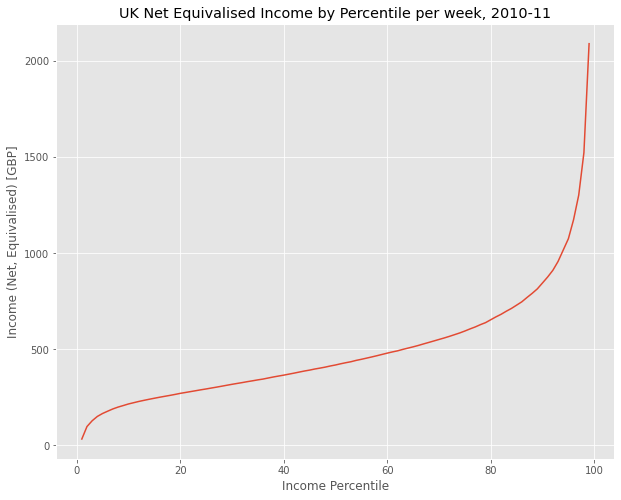
\includegraphics{notebooks/W02. Pandas_files/figure-pdf/cell-13-output-2.png}

}

\end{figure}

We see a curve that is pretty linear in the middle region, but curves
rapidly upwards in the higher percentile and looks more like a power
law.

\hypertarget{exercise-means}{%
\subsection{Exercise: Means}\label{exercise-means}}

Where does the mean appear here? Draw in a horizontal line to show the
mean using \textbf{axhline}. Show the median on the same graph. What is
the meaning of the median in this context?

Hint: Recall that last time we used \emph{axvline} to highlight the mean
and standard deviation by drawing vertical lines on the axis. Here, we
use \emph{axhline} to draw horizontal lines.

\hypertarget{extension-accessing-cells}{%
\subsection{Extension: Accessing
cells}\label{extension-accessing-cells}}

There are a number of ways to access elements of the dataframe: we've
shown how to access columns by the {[}\emph{`name of column'}{]} method,
and rows via the .loc{[}\emph{index}{]} method; and how we can select a
range. There are also .iloc methods to select by number rather than
name; you should become familiar with these on the documentation page
for pandas.

\hypertarget{comparing-segments}{%
\section{Comparing segments}\label{comparing-segments}}

Earlier, we compared some summary statistics of single people and
couples. Let's look at the wider curve for more than one group, now:

\begin{Shaded}
\begin{Highlighting}[]
\CommentTok{\#This is going to throw a load of errors}
\NormalTok{income[[}\StringTok{\textquotesingle{}Single adult\textquotesingle{}}\NormalTok{,}\StringTok{\textquotesingle{}Lone parent, one child under 14\textquotesingle{}}\NormalTok{]].plot()}
\end{Highlighting}
\end{Shaded}

\begin{verbatim}
TypeError: no numeric data to plot
\end{verbatim}

\hypertarget{warning}{%
\section{Warning}\label{warning}}

This isn't looking good. There's a load of text and no graph. If you've
not seen this before, it's an error - something has gone wrong.
Generally, if we look at the \textbf{final} line, it should tell us
what's wrong, in this case there's ``no numeric data to plot'', which is
weird, because we've seen the data and have even plotted some of it.

\hypertarget{messy-data}{%
\section{Messy Data}\label{messy-data}}

DataFrames, as we are starting to see, give us the chance to plot, chop,
slice and data to help us make sense of it. Here, we will create a
\textbf{new} DataFrame to take only two columns of data, and get rid of
any blank cells and any cells which are not being read as numbers -
normally a sign of a missing value or a non-numerical character. Why
could this be happening? It could be

\begin{itemize}
\item
  due to blank spaces in the text file
\item
  due to letters where there should be numbers
\item
  due to characters (``,'', ``-'', etc) that shouldn't really be there
\end{itemize}

In general, there will be some detective work required to figure out
what's wrong in our text file. Your best bet is sometimes to open up the
data in a text editor, like I've done here:

\begin{Shaded}
\begin{Highlighting}[]
\ImportTok{from}\NormalTok{ IPython.display }\ImportTok{import}\NormalTok{ Image}

\NormalTok{data\_path }\OperatorTok{=} \StringTok{"https://s3.eu{-}west{-}2.amazonaws.com/qm2/wk2/data.png"}
\NormalTok{Image(data\_path)}
\end{Highlighting}
\end{Shaded}

\begin{figure}[H]

{\centering 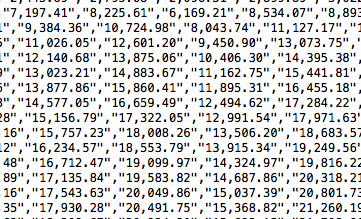
\includegraphics{notebooks/W02. Pandas_files/figure-pdf/cell-15-output-1.png}

}

\end{figure}

That's a screenshot of our datafile, opened up in a text editor. As we
can see, these numbers are separated by commas and surrounded by
quotation marks - this is normal, and what .csv files are supposed to
look like. However, there are a lot of commas within the numbers - which
makes it easier for people to read, but confuses software. Luckily,
Python has a method for dealing with this - the ``replace'' method.

Unfortunately, this dataframe is quite messy, so I'm going to have to
extract just the columns of data I'm interested in to make it work. I'll
do that by creating a new dataframe:

\hypertarget{example-cleaning-data}{%
\section{Example: Cleaning data}\label{example-cleaning-data}}

\begin{Shaded}
\begin{Highlighting}[]
\NormalTok{clean }\OperatorTok{=}\NormalTok{ income[[}\StringTok{\textquotesingle{}Childless couple, annual income\textquotesingle{}}\NormalTok{,}\StringTok{\textquotesingle{}Couple, two children under 14\textquotesingle{}}\NormalTok{]]}
\NormalTok{clean.head()}
\end{Highlighting}
\end{Shaded}

\begin{longtable}[]{@{}lll@{}}
\toprule\noalign{}
& Childless couple, annual income & Couple, two children under 14 \\
Percentile Point & & \\
\midrule\noalign{}
\endhead
\bottomrule\noalign{}
\endlastfoot
1 & 1,746.92 & 2,445.69 \\
2 & 5,141.01 & 7,197.41 \\
3 & 6,703.11 & 9,384.36 \\
4 & 7,875.75 & 11,026.05 \\
5 & 8,671.91 & 12,140.68 \\
\end{longtable}

We see those pesky commas. Now we can get on with cleaning up the data:

\begin{Shaded}
\begin{Highlighting}[]
\NormalTok{clean}\OperatorTok{=}\NormalTok{clean.replace(}\StringTok{\textquotesingle{},\textquotesingle{}}\NormalTok{, }\StringTok{\textquotesingle{}\textquotesingle{}}\NormalTok{, regex}\OperatorTok{=}\VariableTok{True}\NormalTok{)}

\CommentTok{\# In addition, missing values are sometimes written as \textquotesingle{}{-}\textquotesingle{}, in order for Python to understand that it is just a missing numerical }
\CommentTok{\# value, all \textquotesingle{}{-}\textquotesingle{} need to be replaced with \textquotesingle{}NaN\textquotesingle{}.}
\NormalTok{clean }\OperatorTok{=}\NormalTok{ clean.replace(}\StringTok{\textquotesingle{}{-}\textquotesingle{}}\NormalTok{, }\StringTok{\textquotesingle{}NaN\textquotesingle{}}\NormalTok{, regex}\OperatorTok{=}\VariableTok{True}\NormalTok{).astype(}\StringTok{\textquotesingle{}float\textquotesingle{}}\NormalTok{)}
\NormalTok{clean.head()}
\end{Highlighting}
\end{Shaded}

\begin{longtable}[]{@{}lll@{}}
\toprule\noalign{}
& Childless couple, annual income & Couple, two children under 14 \\
Percentile Point & & \\
\midrule\noalign{}
\endhead
\bottomrule\noalign{}
\endlastfoot
1 & 1746.92 & 2445.69 \\
2 & 5141.01 & 7197.41 \\
3 & 6703.11 & 9384.36 \\
4 & 7875.75 & 11026.05 \\
5 & 8671.91 & 12140.68 \\
\end{longtable}

\textbf{Extension}: ``\textbf{Regex}'' refers to ``\textbf{Reg}ular
\textbf{Ex}pression'', which is a way of replacing and cleaning text.
It's a bit beyond the scope of this class, but worth looking into if
you're interested in programming more widely.

This seems to have done the job. We've also put a line in the code to
get rid of dashes - a way that data collectors will sometimes represent
missing data. Now let's plot this.

\hypertarget{asking-more-questions-of-the-data}{%
\section{Asking more questions of the
data}\label{asking-more-questions-of-the-data}}

For me, this data starts to beg further questions. How would we answer
these?

\begin{itemize}
\item
  If the top 20\% of income shows such a sharp increase, how do we know
  that there isn't a similar uptick \emph{within} the 1\%? We've already
  seen that the mean of the dataset as a whole is much less than the
  half the maximum category (it's 25\% of the maximum). What if that's
  true within the 1\%, and £2,000/week as a fraction of the 0.1\%, or
  the 0.01\%?
\item
  How does this break down for gender, or educational background, or
  other factors like ethnicity or country of origin?
\item
  Which parts of the income curve show greater gaps between these
  subgroups and what might it say about the underlying causal
  mechanisms?
\end{itemize}

\begin{Shaded}
\begin{Highlighting}[]
\NormalTok{clean.plot()}
\NormalTok{plt.title(}\StringTok{\textquotesingle{}A Modest Proposal: The fiscal benefits of childbirth\textquotesingle{}}\NormalTok{)}
\NormalTok{plt.xlabel(}\StringTok{\textquotesingle{}Percentile\textquotesingle{}}\NormalTok{)}
\NormalTok{plt.ylabel(}\StringTok{\textquotesingle{}Income Per Week [GBP]\textquotesingle{}}\NormalTok{)}
\end{Highlighting}
\end{Shaded}

\begin{verbatim}
Text(0, 0.5, 'Income Per Week [GBP]')
\end{verbatim}

\begin{figure}[H]

{\centering 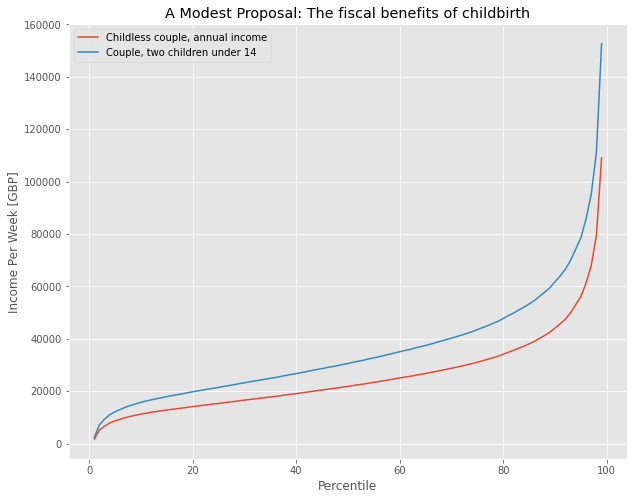
\includegraphics{notebooks/W02. Pandas_files/figure-pdf/cell-18-output-2.png}

}

\end{figure}

\hypertarget{exercise-1}{%
\section{Exercise:}\label{exercise-1}}

Previously, we'd examined income gaps between single people and couples
(how very romantic). Repeat the above exercise (cleaning and plotting
income data) for the columns we used above for single people and
childless couples. Reflect and comment on the differences.

\begin{Shaded}
\begin{Highlighting}[]
\BuiltInTok{print}\NormalTok{(}\StringTok{"Enter your code here"}\NormalTok{)}
\end{Highlighting}
\end{Shaded}

\begin{Shaded}
\begin{Highlighting}[]
\NormalTok{Add your reflection here.}
\end{Highlighting}
\end{Shaded}

So far, we've dealt with selecting data in a particular row of column by
index or label. What if we now want to filter the data by \emph{value}?
For example, let's say I want to see the data for all Childless couples
who earn more than 50,000 (net equivalised) pounds every year. This
looks like:

\begin{Shaded}
\begin{Highlighting}[]
\NormalTok{clean }\OperatorTok{=}\NormalTok{ income[[}\StringTok{\textquotesingle{}Childless couple, annual income\textquotesingle{}}\NormalTok{,}\StringTok{\textquotesingle{}Couple, two children under 14\textquotesingle{}}\NormalTok{]]}
\NormalTok{clean }\OperatorTok{=}\NormalTok{ clean.replace(}\StringTok{\textquotesingle{},\textquotesingle{}}\NormalTok{, }\StringTok{\textquotesingle{}\textquotesingle{}}\NormalTok{, regex}\OperatorTok{=}\VariableTok{True}\NormalTok{)}
\NormalTok{clean }\OperatorTok{=}\NormalTok{ clean.replace(}\StringTok{\textquotesingle{}{-}\textquotesingle{}}\NormalTok{, }\StringTok{\textquotesingle{}NaN\textquotesingle{}}\NormalTok{, regex}\OperatorTok{=}\VariableTok{True}\NormalTok{).astype(}\StringTok{\textquotesingle{}float\textquotesingle{}}\NormalTok{)}
\NormalTok{clean[clean[}\StringTok{\textquotesingle{}Childless couple, annual income\textquotesingle{}}\NormalTok{]}\OperatorTok{\textgreater{}}\DecValTok{50000}\NormalTok{]}
\end{Highlighting}
\end{Shaded}

The key line of code for selection is:

\begin{Shaded}
\begin{Highlighting}[]
\NormalTok{clean[clean[}\StringTok{\textquotesingle{}Childless couple, annual income\textquotesingle{}}\NormalTok{]}\OperatorTok{\textgreater{}}\DecValTok{50000}\NormalTok{]}
\end{Highlighting}
\end{Shaded}

Let's break this down: we're used to using \emph{dataframe}{[}\emph{some
selection}{]} from earlier. Here ``some selection'' is

\begin{Shaded}
\begin{Highlighting}[]
\NormalTok{clean[}\StringTok{\textquotesingle{}Childless couple, annual income\textquotesingle{}}\NormalTok{]}\OperatorTok{\textgreater{}}\DecValTok{50000}
\end{Highlighting}
\end{Shaded}

In other words, this command is returning a set of indices where that
statement is true. We can see this explicitly:

\begin{Shaded}
\begin{Highlighting}[]
\NormalTok{clean[}\StringTok{\textquotesingle{}Childless couple, annual income\textquotesingle{}}\NormalTok{]}\OperatorTok{\textgreater{}}\DecValTok{50000}
\end{Highlighting}
\end{Shaded}

So python is picking the values where this statement is true -
i.e.~where the `Childless couple\ldots{}' column has values greater than
50000. Then this selection is passed to the dataframe, and the dataframe
shows the correct rows.

We won't dwell on comparative operative, here we've used
``\textgreater{}'' to mean ``is greater than''; you can also use:

\begin{itemize}
\tightlist
\item
  == to mean `is equal to' {[}why the double equals?{]}
\item
  \textless\textgreater{} or != to mean `is not equal to'
\item
  \textless{} to mean `is less than'
\item
  the symbol \textgreater= to mean `is greater than or equal to'
\item
  \textless= to mean `is less than or equal to'
\end{itemize}

\hypertarget{exercise-2}{%
\section{Exercise}\label{exercise-2}}

On an approporiately labelled graph, plot the incomes of all single
adults whose net equivalised income is less than or equal to £10,000.
What proportion of the population is this?

\bookmarksetup{startatroot}

\hypertarget{extension-web-scraping}{%
\chapter{Extension: Web Scraping}\label{extension-web-scraping}}

In this example, we've been working with a .csv file that contains all
the data we want. That's not always the case. Let's say we're interested
in getting the data from a table on a website. Websites are built using
HTML code, so what we need to figure out how to look inside the
website's code and pull out the data we want. Luckily, pandas has a
built in function that can automatically recognize HTML tables in
websites and turn them into dataframes.

Let's start with the \href{https://top10.netflix.com/}{Netflix Top 10}
website. Click on the link and have a look around. You'll notice two
tables: the first showing the top 10 films this week, and the second
(farther down) showing the most popular filsms based on their first 28
days on netflix.

We can download both of these tables into python using one pandas
function: read\_html

\begin{Shaded}
\begin{Highlighting}[]
\NormalTok{url}\OperatorTok{=}\StringTok{\textquotesingle{}https://top10.netflix.com/\textquotesingle{}}

\NormalTok{tables}\OperatorTok{=}\NormalTok{pandas.read\_html(url)}

\BuiltInTok{print}\NormalTok{(tables)}
\end{Highlighting}
\end{Shaded}

\begin{verbatim}
[    #  \
0   1   
1   2   
2   3   
3   4   
4   5   
5   6   
6   7   
7   8   
8   9   
9  10   

  .css-ld8rqy-container{position:relative;box-sizing:border-box;min-width:0;}.css-7pg0cj-a11yText{z-index:9999;border:0;clip:rect(1px, 1px, 1px, 1px);height:1px;width:1px;position:absolute;overflow:hidden;padding:0;white-space:nowrap;}.css-3zcu7z-control{-webkit-align-items:center;-webkit-box-align:center;-ms-flex-align:center;align-items:center;background-color:hsl(0, 0%, 100%);border-color:hsl(0, 0%, 80%);border-radius:0;border-style:solid;border-width:1px;box-shadow:none;cursor:pointer;display:-webkit-box;display:-webkit-flex;display:-ms-flexbox;display:flex;-webkit-box-flex-wrap:wrap;-webkit-flex-wrap:wrap;-ms-flex-wrap:wrap;flex-wrap:wrap;-webkit-box-pack:justify;-webkit-justify-content:space-between;justify-content:space-between;min-height:0rem;outline:0!important;position:relative;-webkit-transition:all 100ms;transition:all 100ms;box-sizing:border-box;background:transparent;border:none;padding:0px 3px;margin-left:-5px;}.css-3zcu7z-control:hover{border-color:rgba(255,255,255,0.9);}.css-zl2g27{-webkit-align-items:center;-webkit-box-align:center;-ms-flex-align:center;align-items:center;display:grid;-webkit-flex:1;-ms-flex:1;flex:1;-webkit-box-flex-wrap:wrap;-webkit-flex-wrap:wrap;-ms-flex-wrap:wrap;flex-wrap:wrap;padding:0;-webkit-overflow-scrolling:touch;position:relative;overflow:hidden;box-sizing:border-box;}.css-hlu0h4-singleValue{color:white;grid-area:1/1/2/3;margin-left:2px;margin-right:2px;max-width:100%;overflow:hidden;text-overflow:ellipsis;white-space:nowrap;box-sizing:border-box;}Films (English).css-1a9ai41{margin:0;padding-bottom:2px;padding-top:2px;visibility:visible;color:hsl(0, 0%, 20%);-webkit-flex:1 1 auto;-ms-flex:1 1 auto;flex:1 1 auto;display:inline-grid;grid-area:1/1/2/3;grid-template-columns:0 min-content;box-sizing:border-box;padding:0;}.css-1a9ai41:after{content:attr(data-value) " ";visibility:hidden;white-space:pre;grid-area:1/2;font:inherit;min-width:2px;border:0;margin:0;outline:0;padding:0;}.css-1wy0on6{-webkit-align-items:center;-webkit-box-align:center;-ms-flex-align:center;align-items:center;-webkit-align-self:stretch;-ms-flex-item-align:stretch;align-self:stretch;display:-webkit-box;display:-webkit-flex;display:-ms-flexbox;display:flex;-webkit-flex-shrink:0;-ms-flex-negative:0;flex-shrink:0;box-sizing:border-box;}.css-1hyfx7x{display:none;}.css-xhbtlw-indicatorContainer{color:hsl(0, 0%, 80%);display:-webkit-box;display:-webkit-flex;display:-ms-flexbox;display:flex;padding:8px;-webkit-transition:color 150ms;transition:color 150ms;box-sizing:border-box;-webkit-transform:scale(0.8);-moz-transform:scale(0.8);-ms-transform:scale(0.8);transform:scale(0.8);}.css-xhbtlw-indicatorContainer:hover{color:hsl(0, 0%, 60%);}.css-xhbtlw-indicatorContainer:hover{-webkit-transform:scale(1);-moz-transform:scale(1);-ms-transform:scale(1);transform:scale(1);}  \
0                                Luckiest Girl Alive                                                                                                                                                                                                                                                                                                                                                                                                                                                                                                                                                                                                                                                                                                                                                                                                                                                                                                                                                                                                                                                                                                                                                                                                                                                                                                                                                                                                                                                                                                                                                                                                                                                                                                                                                                                                                                                                                                                                                                                                                                                                                                                                                                                                                                                                                                                                                                                                                                                                                                                                                                                                                                                                                                                                                                                                                                                                                       
1                               Mr. Harrigan's Phone                                                                                                                                                                                                                                                                                                                                                                                                                                                                                                                                                                                                                                                                                                                                                                                                                                                                                                                                                                                                                                                                                                                                                                                                                                                                                                                                                                                                                                                                                                                                                                                                                                                                                                                                                                                                                                                                                                                                                                                                                                                                                                                                                                                                                                                                                                                                                                                                                                                                                                                                                                                                                                                                                                                                                                                                                                                                                       
2                                    Last Seen Alive                                                                                                                                                                                                                                                                                                                                                                                                                                                                                                                                                                                                                                                                                                                                                                                                                                                                                                                                                                                                                                                                                                                                                                                                                                                                                                                                                                                                                                                                                                                                                                                                                                                                                                                                                                                                                                                                                                                                                                                                                                                                                                                                                                                                                                                                                                                                                                                                                                                                                                                                                                                                                                                                                                                                                                                                                                                                                       
3                                             Blonde                                                                                                                                                                                                                                                                                                                                                                                                                                                                                                                                                                                                                                                                                                                                                                                                                                                                                                                                                                                                                                                                                                                                                                                                                                                                                                                                                                                                                                                                                                                                                                                                                                                                                                                                                                                                                                                                                                                                                                                                                                                                                                                                                                                                                                                                                                                                                                                                                                                                                                                                                                                                                                                                                                                                                                                                                                                                                       
4                                                Lou                                                                                                                                                                                                                                                                                                                                                                                                                                                                                                                                                                                                                                                                                                                                                                                                                                                                                                                                                                                                                                                                                                                                                                                                                                                                                                                                                                                                                                                                                                                                                                                                                                                                                                                                                                                                                                                                                                                                                                                                                                                                                                                                                                                                                                                                                                                                                                                                                                                                                                                                                                                                                                                                                                                                                                                                                                                                                       
5                                      The Boss Baby                                                                                                                                                                                                                                                                                                                                                                                                                                                                                                                                                                                                                                                                                                                                                                                                                                                                                                                                                                                                                                                                                                                                                                                                                                                                                                                                                                                                                                                                                                                                                                                                                                                                                                                                                                                                                                                                                                                                                                                                                                                                                                                                                                                                                                                                                                                                                                                                                                                                                                                                                                                                                                                                                                                                                                                                                                                                                       
6                                               Sing                                                                                                                                                                                                                                                                                                                                                                                                                                                                                                                                                                                                                                                                                                                                                                                                                                                                                                                                                                                                                                                                                                                                                                                                                                                                                                                                                                                                                                                                                                                                                                                                                                                                                                                                                                                                                                                                                                                                                                                                                                                                                                                                                                                                                                                                                                                                                                                                                                                                                                                                                                                                                                                                                                                                                                                                                                                                                       
7                                          Marauders                                                                                                                                                                                                                                                                                                                                                                                                                                                                                                                                                                                                                                                                                                                                                                                                                                                                                                                                                                                                                                                                                                                                                                                                                                                                                                                                                                                                                                                                                                                                                                                                                                                                                                                                                                                                                                                                                                                                                                                                                                                                                                                                                                                                                                                                                                                                                                                                                                                                                                                                                                                                                                                                                                                                                                                                                                                                                       
8                                    The Redeem Team                                                                                                                                                                                                                                                                                                                                                                                                                                                                                                                                                                                                                                                                                                                                                                                                                                                                                                                                                                                                                                                                                                                                                                                                                                                                                                                                                                                                                                                                                                                                                                                                                                                                                                                                                                                                                                                                                                                                                                                                                                                                                                                                                                                                                                                                                                                                                                                                                                                                                                                                                                                                                                                                                                                                                                                                                                                                                       
9                            Minions & More Volume 1                                                                                                                                                                                                                                                                                                                                                                                                                                                                                                                                                                                                                                                                                                                                                                                                                                                                                                                                                                                                                                                                                                                                                                                                                                                                                                                                                                                                                                                                                                                                                                                                                                                                                                                                                                                                                                                                                                                                                                                                                                                                                                                                                                                                                                                                                                                                                                                                                                                                                                                                                                                                                                                                                                                                                                                                                                                                                       

   Weeks in Top 10  Hours viewed  
0                1      43080000  
1                1      35420000  
2                2      18810000  
3                2      17410000  
4                3      12600000  
5                1       8510000  
6                1       8420000  
7                2       8350000  
8                1       7850000  
9                3       7090000  ,     #  \
0   1   
1   2   
2   3   
3   4   
4   5   
5   6   
6   7   
7   8   
8   9   
9  10   

  .css-ld8rqy-container{position:relative;box-sizing:border-box;min-width:0;}.css-7pg0cj-a11yText{z-index:9999;border:0;clip:rect(1px, 1px, 1px, 1px);height:1px;width:1px;position:absolute;overflow:hidden;padding:0;white-space:nowrap;}.css-3zcu7z-control{-webkit-align-items:center;-webkit-box-align:center;-ms-flex-align:center;align-items:center;background-color:hsl(0, 0%, 100%);border-color:hsl(0, 0%, 80%);border-radius:0;border-style:solid;border-width:1px;box-shadow:none;cursor:pointer;display:-webkit-box;display:-webkit-flex;display:-ms-flexbox;display:flex;-webkit-box-flex-wrap:wrap;-webkit-flex-wrap:wrap;-ms-flex-wrap:wrap;flex-wrap:wrap;-webkit-box-pack:justify;-webkit-justify-content:space-between;justify-content:space-between;min-height:0rem;outline:0!important;position:relative;-webkit-transition:all 100ms;transition:all 100ms;box-sizing:border-box;background:transparent;border:none;padding:0px 3px;margin-left:-5px;}.css-3zcu7z-control:hover{border-color:rgba(255,255,255,0.9);}.css-zl2g27{-webkit-align-items:center;-webkit-box-align:center;-ms-flex-align:center;align-items:center;display:grid;-webkit-flex:1;-ms-flex:1;flex:1;-webkit-box-flex-wrap:wrap;-webkit-flex-wrap:wrap;-ms-flex-wrap:wrap;flex-wrap:wrap;padding:0;-webkit-overflow-scrolling:touch;position:relative;overflow:hidden;box-sizing:border-box;}.css-hlu0h4-singleValue{color:white;grid-area:1/1/2/3;margin-left:2px;margin-right:2px;max-width:100%;overflow:hidden;text-overflow:ellipsis;white-space:nowrap;box-sizing:border-box;}Films (English).css-1a9ai41{margin:0;padding-bottom:2px;padding-top:2px;visibility:visible;color:hsl(0, 0%, 20%);-webkit-flex:1 1 auto;-ms-flex:1 1 auto;flex:1 1 auto;display:inline-grid;grid-area:1/1/2/3;grid-template-columns:0 min-content;box-sizing:border-box;padding:0;}.css-1a9ai41:after{content:attr(data-value) " ";visibility:hidden;white-space:pre;grid-area:1/2;font:inherit;min-width:2px;border:0;margin:0;outline:0;padding:0;}.css-1wy0on6{-webkit-align-items:center;-webkit-box-align:center;-ms-flex-align:center;align-items:center;-webkit-align-self:stretch;-ms-flex-item-align:stretch;align-self:stretch;display:-webkit-box;display:-webkit-flex;display:-ms-flexbox;display:flex;-webkit-flex-shrink:0;-ms-flex-negative:0;flex-shrink:0;box-sizing:border-box;}.css-1hyfx7x{display:none;}.css-xhbtlw-indicatorContainer{color:hsl(0, 0%, 80%);display:-webkit-box;display:-webkit-flex;display:-ms-flexbox;display:flex;padding:8px;-webkit-transition:color 150ms;transition:color 150ms;box-sizing:border-box;-webkit-transform:scale(0.8);-moz-transform:scale(0.8);-ms-transform:scale(0.8);transform:scale(0.8);}.css-xhbtlw-indicatorContainer:hover{color:hsl(0, 0%, 60%);}.css-xhbtlw-indicatorContainer:hover{-webkit-transform:scale(1);-moz-transform:scale(1);-ms-transform:scale(1);transform:scale(1);}  \
0                                         Red Notice                                                                                                                                                                                                                                                                                                                                                                                                                                                                                                                                                                                                                                                                                                                                                                                                                                                                                                                                                                                                                                                                                                                                                                                                                                                                                                                                                                                                                                                                                                                                                                                                                                                                                                                                                                                                                                                                                                                                                                                                                                                                                                                                                                                                                                                                                                                                                                                                                                                                                                                                                                                                                                                                                                                                                                                                                                                                                       
1                                      Don't Look Up                                                                                                                                                                                                                                                                                                                                                                                                                                                                                                                                                                                                                                                                                                                                                                                                                                                                                                                                                                                                                                                                                                                                                                                                                                                                                                                                                                                                                                                                                                                                                                                                                                                                                                                                                                                                                                                                                                                                                                                                                                                                                                                                                                                                                                                                                                                                                                                                                                                                                                                                                                                                                                                                                                                                                                                                                                                                                       
2                                           Bird Box                                                                                                                                                                                                                                                                                                                                                                                                                                                                                                                                                                                                                                                                                                                                                                                                                                                                                                                                                                                                                                                                                                                                                                                                                                                                                                                                                                                                                                                                                                                                                                                                                                                                                                                                                                                                                                                                                                                                                                                                                                                                                                                                                                                                                                                                                                                                                                                                                                                                                                                                                                                                                                                                                                                                                                                                                                                                                       
3                                       The Gray Man                                                                                                                                                                                                                                                                                                                                                                                                                                                                                                                                                                                                                                                                                                                                                                                                                                                                                                                                                                                                                                                                                                                                                                                                                                                                                                                                                                                                                                                                                                                                                                                                                                                                                                                                                                                                                                                                                                                                                                                                                                                                                                                                                                                                                                                                                                                                                                                                                                                                                                                                                                                                                                                                                                                                                                                                                                                                                       
4                                   The Adam Project                                                                                                                                                                                                                                                                                                                                                                                                                                                                                                                                                                                                                                                                                                                                                                                                                                                                                                                                                                                                                                                                                                                                                                                                                                                                                                                                                                                                                                                                                                                                                                                                                                                                                                                                                                                                                                                                                                                                                                                                                                                                                                                                                                                                                                                                                                                                                                                                                                                                                                                                                                                                                                                                                                                                                                                                                                                                                       
5                                         Extraction                                                                                                                                                                                                                                                                                                                                                                                                                                                                                                                                                                                                                                                                                                                                                                                                                                                                                                                                                                                                                                                                                                                                                                                                                                                                                                                                                                                                                                                                                                                                                                                                                                                                                                                                                                                                                                                                                                                                                                                                                                                                                                                                                                                                                                                                                                                                                                                                                                                                                                                                                                                                                                                                                                                                                                                                                                                                                       
6                                      Purple Hearts                                                                                                                                                                                                                                                                                                                                                                                                                                                                                                                                                                                                                                                                                                                                                                                                                                                                                                                                                                                                                                                                                                                                                                                                                                                                                                                                                                                                                                                                                                                                                                                                                                                                                                                                                                                                                                                                                                                                                                                                                                                                                                                                                                                                                                                                                                                                                                                                                                                                                                                                                                                                                                                                                                                                                                                                                                                                                       
7                                   The Unforgivable                                                                                                                                                                                                                                                                                                                                                                                                                                                                                                                                                                                                                                                                                                                                                                                                                                                                                                                                                                                                                                                                                                                                                                                                                                                                                                                                                                                                                                                                                                                                                                                                                                                                                                                                                                                                                                                                                                                                                                                                                                                                                                                                                                                                                                                                                                                                                                                                                                                                                                                                                                                                                                                                                                                                                                                                                                                                                       
8                                       The Irishman                                                                                                                                                                                                                                                                                                                                                                                                                                                                                                                                                                                                                                                                                                                                                                                                                                                                                                                                                                                                                                                                                                                                                                                                                                                                                                                                                                                                                                                                                                                                                                                                                                                                                                                                                                                                                                                                                                                                                                                                                                                                                                                                                                                                                                                                                                                                                                                                                                                                                                                                                                                                                                                                                                                                                                                                                                                                                       
9                                The Kissing Booth 2                                                                                                                                                                                                                                                                                                                                                                                                                                                                                                                                                                                                                                                                                                                                                                                                                                                                                                                                                                                                                                                                                                                                                                                                                                                                                                                                                                                                                                                                                                                                                                                                                                                                                                                                                                                                                                                                                                                                                                                                                                                                                                                                                                                                                                                                                                                                                                                                                                                                                                                                                                                                                                                                                                                                                                                                                                                                                       

   Hours viewed in first 28 days  
0                      364020000  
1                      359790000  
2                      282020000  
3                      253870000  
4                      233160000  
5                      231340000  
6                      228690000  
7                      214700000  
8                      214570000  
9                      209250000  ]
\end{verbatim}

When we print the results of what was scraped, it's pretty ugly. One of
the reasons is that the \texttt{tables} variable is actually a
\emph{list} of dataframes. Because there were two tables on our website,
\texttt{read\_html} has returned both of those tables and put them in a
list. let's save the first table as a new dataframe called
\texttt{top10} and have a closer look.

\begin{Shaded}
\begin{Highlighting}[]
\NormalTok{top10}\OperatorTok{=}\NormalTok{tables[}\DecValTok{0}\NormalTok{]}
\NormalTok{top10}
\end{Highlighting}
\end{Shaded}

This looks more like the dataframes we were looking at earlier. There's
a big chunk of text (this is HTML code, the language websites are built
with) where the name of the second column should be. \texttt{read\_html}
is usually pretty smart, and can actually read the column names from the
tables on the website. It seems to have gotten confused for this one
column. If we print the columns from the We can rename that column using
the \texttt{rename} function. Since we know it's the second column, we
can select it with \texttt{top10.columns{[}1{]}}

\begin{Shaded}
\begin{Highlighting}[]
\NormalTok{top10.rename(columns}\OperatorTok{=}\NormalTok{\{top10.columns[}\DecValTok{1}\NormalTok{]: }\StringTok{"Title"}\NormalTok{ \}, inplace }\OperatorTok{=} \VariableTok{True}\NormalTok{)}
\NormalTok{top10}
\end{Highlighting}
\end{Shaded}

And there we have it; a nicely formatted dataframe ready for analysis,
straight from a website.

\bookmarksetup{startatroot}

\hypertarget{assessed-question-1}{%
\chapter{Assessed Question}\label{assessed-question-1}}

Using the following URL
https://en.wikipedia.org/wiki/List\_of\_Nobel\_laureates\_in\_Chemistry
create a plot of the top 10 countries in terms of nobel laureates.
First, follow the steps below:

\begin{Shaded}
\begin{Highlighting}[]
\CommentTok{\# scrape the table of Nobel Laureates in Chemistry using read\_html. remember, this gives us a LIST of dataframes! lets call this list chem\_tables}

\CommentTok{\# select the first dataframe from this list and call it chem}
\end{Highlighting}
\end{Shaded}

I'll help you out with this next bit. We'll be using the
\texttt{groupby} function in pandas to group our dataframe such that
each row is a country (rather than a person, as it currently is). We do
this by using
\texttt{\textless{}dataframe\textgreater{}.groupby(\textquotesingle{}\textless{}column\ name\textgreater{}\textquotesingle{})}.
Since we're aggregating, we need to tell python how we want it to
aggregate our values. In this case, we just want to count the number of
rows for each country; we can do this using \texttt{.size()}. You can
use many different aggregation functions, e.g.~\texttt{.mean()} if you
wanted to calculate the average of a specific column.

\begin{Shaded}
\begin{Highlighting}[]
\CommentTok{\# create a new dataframe called \textquotesingle{}country\textquotesingle{} in which each row is a country, and the values represent the number of nobel laureates. }

\CommentTok{\# now sort it in descending order}

\CommentTok{\# finally, plot the top 10 countries }
\end{Highlighting}
\end{Shaded}

\emph{QUESTION: What country has the sixth most nobel prizes in
chemistry?}

\bookmarksetup{startatroot}

\hypertarget{spatiotemporal-data}{%
\chapter{Spatiotemporal Data}\label{spatiotemporal-data}}

\hypertarget{workshop-3-open-in-colab}{%
\section[\emph{Workshop 3} ]{\texorpdfstring{\emph{Workshop 3}
\href{https://colab.research.google.com/github/oballinger/QM2/blob/main/notebooks/W03.\%20Spatial\%20Data.ipynb}{\protect
\includegraphics{index_files/mediabag/colab-badge.png}}}{Workshop 3 Open In Colab}}\label{workshop-3-open-in-colab}}

Sometimes the data we work with references points on the earth's
surface, unlocking a rich set of analytical possibilities. In today's
workshop, we're going to be exploring the effect of the 2020 California
Wildfires on air quality across the state. We'll be using real air
quality data collected by sensors and combining it with satellite
imagery to show how toxic smoke from wildfires swept over America's
largest state.

\hypertarget{aims-1}{%
\subsection{Aims}\label{aims-1}}

\begin{itemize}
\tightlist
\item
  Understanding spatiotemporal data
\item
  Grouping data in pandas
\item
  Manipulating and plotting geographic data
\end{itemize}

\hypertarget{background}{%
\section{Background}\label{background}}

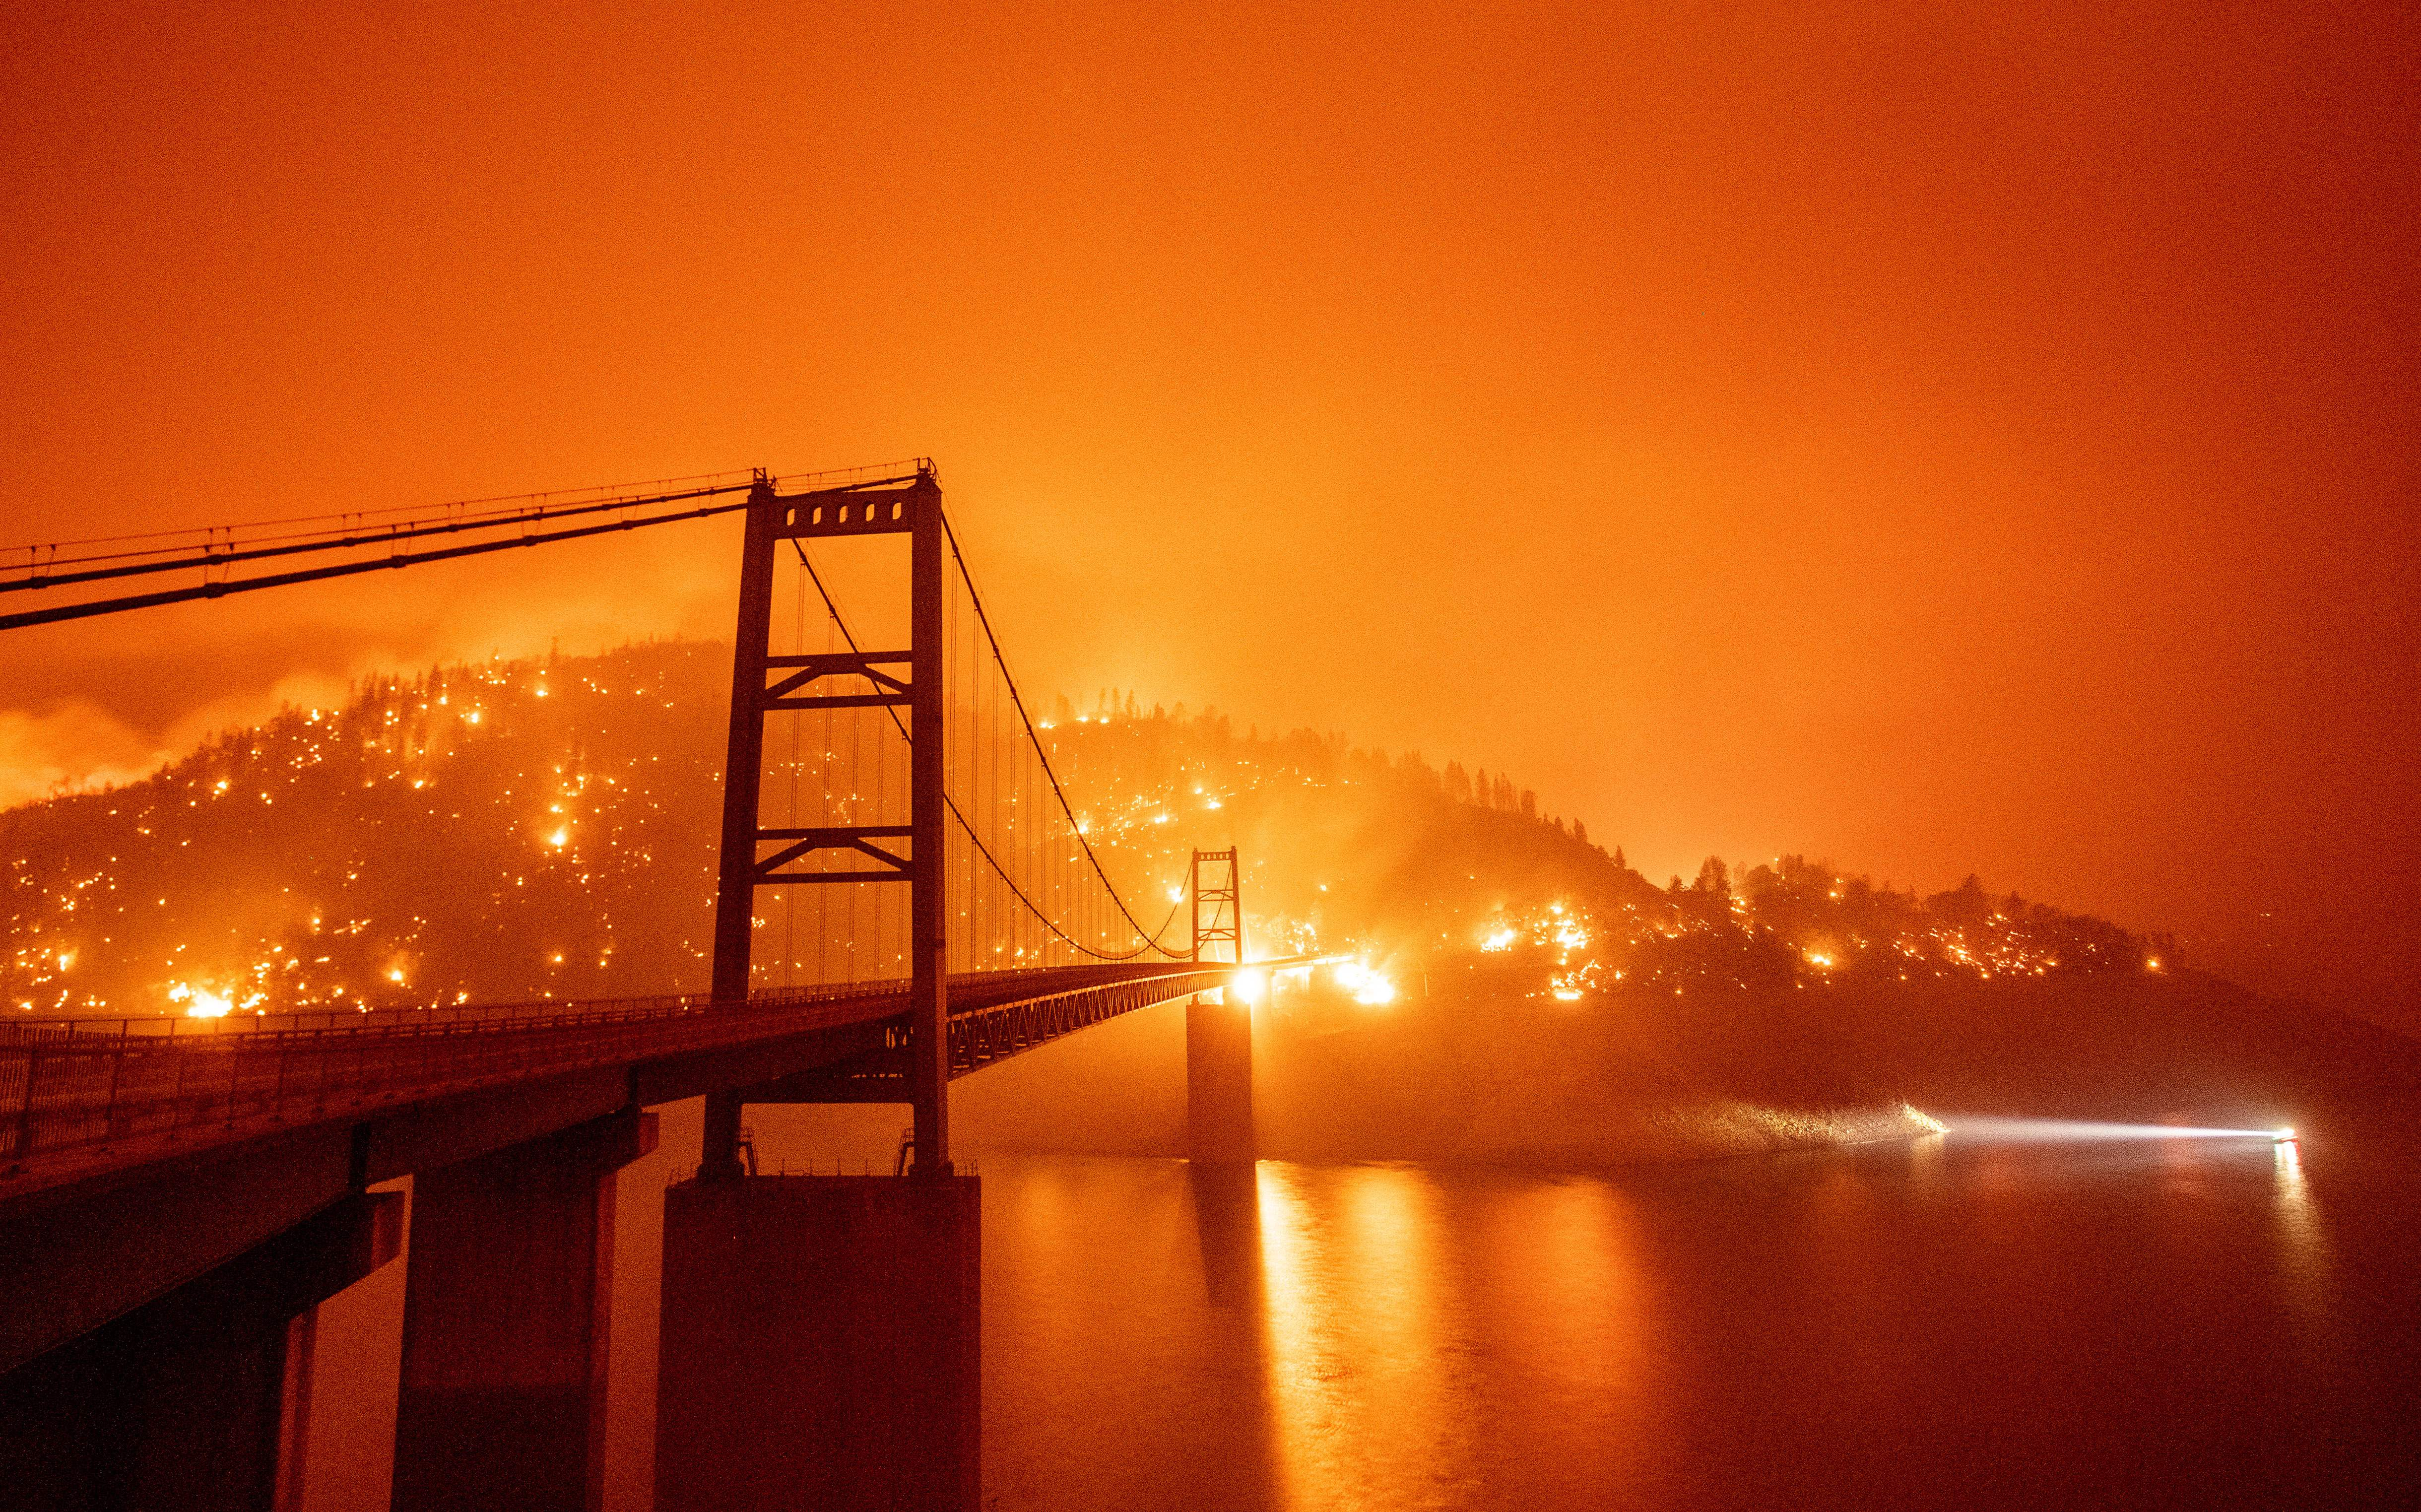
\includegraphics{index_files/mediabag/106695701-1599664926.jpg}

The \href{https://en.wikipedia.org/wiki/2020_California_wildfires}{2020
California wildfire season} was record-setting. By the end of the year,
9,917 fires had burned more than 4\% of the state's area, making 2020
the largest wildfire season recorded in California's modern history.
California's August Complex fire has been described as the first
``gigafire'', burning over 1 million acres across seven counties, an
area larger than the state of Rhode Island. The fires destroyed over
10,000 structures and cost over \$12.079 billion (2020 USD) in damages,
including over \$10 billion in property damage and \$2.079 billion in
fire suppression costs. The intensity of the fire season has been
attributed to a combination of more than a century of poor forest
management and higher temperatures resulting from climate change.

The fires also had a
\href{https://epic.uchicago.edu/news/pollution-from-californias-2020-wildfires-likely-offset-decades-of-air-quality-gains/}{profound
effect on air quality}: ``Places that are experiencing frequent or more
frequent wildfires are going to experience higher air pollution levels,
not just for a couple of days or weeks, but it could impact the annual
level of exposure,'' said Christa Hasenkopf, director of air quality
programs at the University of Chicago institute. ``It can bump up that
average to unsafe and unhealthy levels that really do have an impact on
people's health. When we think of wildfires, we think of short-term
events --- and hopefully they are --- but they can have long-term
consequences considering your overall air pollution exposure.''

\hypertarget{getting-started}{%
\section{Getting Started}\label{getting-started}}

Let's begin by installing some libraries that we'll be working with
today.

\begin{Shaded}
\begin{Highlighting}[]
\OperatorTok{\%\%}\NormalTok{capture}
\OperatorTok{!}\NormalTok{pip install Basemap}
\OperatorTok{!}\NormalTok{pip install ipyleaflet}
\end{Highlighting}
\end{Shaded}

\hypertarget{importing-libraries}{%
\section{Importing Libraries}\label{importing-libraries}}

The first step in any python script is to import the necessary
libraries:

\begin{Shaded}
\begin{Highlighting}[]
\ImportTok{import}\NormalTok{ pandas }\ImportTok{as}\NormalTok{ pd}
\ImportTok{import}\NormalTok{ matplotlib}
\ImportTok{import}\NormalTok{ matplotlib.pyplot }\ImportTok{as}\NormalTok{ plt}
\ImportTok{import}\NormalTok{ numpy }\ImportTok{as}\NormalTok{ np}
\ImportTok{import}\NormalTok{ pylab}
\ImportTok{from}\NormalTok{ datetime }\ImportTok{import}\NormalTok{ datetime}

\OperatorTok{\%}\NormalTok{matplotlib inline}
\NormalTok{pylab.rcParams[}\StringTok{\textquotesingle{}figure.figsize\textquotesingle{}}\NormalTok{] }\OperatorTok{=}\NormalTok{ (}\DecValTok{10}\NormalTok{, }\DecValTok{8}\NormalTok{)}
\end{Highlighting}
\end{Shaded}

\hypertarget{downloading-data-1}{%
\section{Downloading Data}\label{downloading-data-1}}

The next step is to import the data that we need for our analysis. This
week we'll be using real data collected in 2020 by the
\href{https://www.epa.gov/outdoor-air-quality-data/download-daily-data}{Environmental
Protection Agency (EPA)}. I've generated a .csv file containing the data
that I want using the dropdown menus. The EPA also has an
\href{https://aqs.epa.gov/aqsweb/documents/data_api.html}{Application
Programming Interface} for air quality data, which you could use to pull
in data directly into python without having to download a .csv!

Let's open the .csv file and have a look at it:

\begin{Shaded}
\begin{Highlighting}[]
\NormalTok{df}\OperatorTok{=}\NormalTok{pd.read\_csv(}\StringTok{\textquotesingle{}https://qm2.s3.eu{-}west{-}2.amazonaws.com/wk3/california\_aqi.csv\textquotesingle{}}\NormalTok{)}
\NormalTok{df}
\end{Highlighting}
\end{Shaded}

\begin{longtable}[]{@{}lllllllllll@{}}
\toprule\noalign{}
& Date & Site ID & POC & PM & AQI & Site Name & CBSA\_NAME & COUNTY &
latitude & longitude \\
\midrule\noalign{}
\endhead
\bottomrule\noalign{}
\endlastfoot
0 & 1/1/20 & 60010007 & 3 & 8.6 & 36 & Livermore & San
Francisco-Oakland-Hayward, CA & Alameda & 37.687526 & -121.784217 \\
1 & 1/2/20 & 60010007 & 3 & 4.5 & 19 & Livermore & San
Francisco-Oakland-Hayward, CA & Alameda & 37.687526 & -121.784217 \\
2 & 1/3/20 & 60010007 & 3 & 14.2 & 55 & Livermore & San
Francisco-Oakland-Hayward, CA & Alameda & 37.687526 & -121.784217 \\
3 & 1/4/20 & 60010007 & 3 & 10.9 & 45 & Livermore & San
Francisco-Oakland-Hayward, CA & Alameda & 37.687526 & -121.784217 \\
4 & 1/5/20 & 60010007 & 3 & 7.8 & 33 & Livermore & San
Francisco-Oakland-Hayward, CA & Alameda & 37.687526 & -121.784217 \\
... & ... & ... & ... & ... & ... & ... & ... & ... & ... & ... \\
55686 & 11/29/20 & 61131003 & 1 & 20.3 & 68 & Woodland-Gibson Road &
Sacramento-\/-Roseville-\/-Arden-Arcade, CA & Yolo & 38.661210 &
-121.732690 \\
55687 & 12/18/20 & 61131003 & 1 & 2.8 & 12 & Woodland-Gibson Road &
Sacramento-\/-Roseville-\/-Arden-Arcade, CA & Yolo & 38.661210 &
-121.732690 \\
55688 & 12/20/20 & 61131003 & 1 & 22.4 & 73 & Woodland-Gibson Road &
Sacramento-\/-Roseville-\/-Arden-Arcade, CA & Yolo & 38.661210 &
-121.732690 \\
55689 & 12/23/20 & 61131003 & 1 & 11.8 & 49 & Woodland-Gibson Road &
Sacramento-\/-Roseville-\/-Arden-Arcade, CA & Yolo & 38.661210 &
-121.732690 \\
55690 & 12/29/20 & 61131003 & 1 & 5.6 & 23 & Woodland-Gibson Road &
Sacramento-\/-Roseville-\/-Arden-Arcade, CA & Yolo & 38.661210 &
-121.732690 \\
\end{longtable}

Each row in this dataset is an individual reading from an air quality
sensor. The first row is a reading from sensor number 60010007 on
January 1st 2020. It is located in Alameda County, and recorded an Air
Quality Index (AQI) reading of 36. So for each sensor (uniquely
identified by the Site ID column) we will have 365 readings. We also
have the latitude and longitude of each one of these air quality
sensors. The presence of these fields makes this
\textbf{spatio-temporal} data. We'll first analyze the temporal
dimension of our data, before adding in the spatial dimension

\hypertarget{temporal-data}{%
\section{Temporal Data}\label{temporal-data}}

Before we go any further, we need to focus on a very special column in
our dataset: the ``Date'' column. We'll be relying heavily on this
dimension of our dataset. Whenever we have temporal data, the first
thing we want to do is check whether pandas is storing it as datetime
information or as a string (text). We can do this using the
\texttt{dtype} function.

\begin{Shaded}
\begin{Highlighting}[]
\BuiltInTok{print}\NormalTok{(}\StringTok{\textquotesingle{}Prior to cleaning, the data type of the "Date" column is:\textquotesingle{}}\NormalTok{, df[}\StringTok{\textquotesingle{}Date\textquotesingle{}}\NormalTok{].dtype)}

\NormalTok{df[}\StringTok{\textquotesingle{}Date\textquotesingle{}}\NormalTok{]}\OperatorTok{=}\NormalTok{pd.to\_datetime(df[}\StringTok{\textquotesingle{}Date\textquotesingle{}}\NormalTok{])}

\BuiltInTok{print}\NormalTok{(}\StringTok{\textquotesingle{}Now, it is stored as: \textquotesingle{}}\NormalTok{, df[}\StringTok{\textquotesingle{}Date\textquotesingle{}}\NormalTok{].dtype)}
\end{Highlighting}
\end{Shaded}

\begin{verbatim}
Prior to cleaning, the data type of the "Date" column is: object
Now, it is stored as:  datetime64[ns]
\end{verbatim}

Once we've stored the Date column as datetime information, we can do all
sorts of useful things with it. For example, we can quickly extract the
month from the date, or even the ``day of year'' (i.e., how many days
since January 1st of that year have passed). Try doing that in one line
of code if your ``Date'' column is stored as text!

\begin{Shaded}
\begin{Highlighting}[]
\CommentTok{\# we can extract the month from the Date column and save it as a new column }
\NormalTok{df[}\StringTok{\textquotesingle{}Month\textquotesingle{}}\NormalTok{]}\OperatorTok{=}\NormalTok{df[}\StringTok{\textquotesingle{}Date\textquotesingle{}}\NormalTok{].dt.month}
\CommentTok{\# we can do the same for the day of year. }
\NormalTok{df[}\StringTok{\textquotesingle{}Day\textquotesingle{}}\NormalTok{]}\OperatorTok{=}\NormalTok{df[}\StringTok{\textquotesingle{}Date\textquotesingle{}}\NormalTok{].dt.dayofyear}

\BuiltInTok{print}\NormalTok{(df[[}\StringTok{\textquotesingle{}Date\textquotesingle{}}\NormalTok{,}\StringTok{\textquotesingle{}Month\textquotesingle{}}\NormalTok{,}\StringTok{\textquotesingle{}Day\textquotesingle{}}\NormalTok{]])}
\end{Highlighting}
\end{Shaded}

\begin{verbatim}
            Date  Month  Day
0     2020-01-01      1    1
1     2020-01-02      1    2
2     2020-01-03      1    3
3     2020-01-04      1    4
4     2020-01-05      1    5
...          ...    ...  ...
55686 2020-11-29     11  334
55687 2020-12-18     12  353
55688 2020-12-20     12  355
55689 2020-12-23     12  358
55690 2020-12-29     12  364

[55691 rows x 3 columns]
\end{verbatim}

When I print the new columns we've made (``Month'' and ``Day'') next to
the original ``Date'' column, we can see that everything is working as
it should. First date (January 1st, 2020), has a value of 1 in the month
column, and a 1 in the day column. The last row in the dataset was a
sensor reading raken on December 29th, 2020. It has a month of 12, and
day-of-year value of 364. Great.

\hypertarget{exercise-3}{%
\subsection{Exercise}\label{exercise-3}}

\href{https://pandas.pydata.org/docs/reference/api/pandas.Series.dt.dayofyear.html}{Here's}
the documentation for the pandas function that allowed us to extract the
day of year from the datetime column. Using the documentation on this
page, create a new column in the dataframe that contains the week of
year.

\hypertarget{grouping-data}{%
\subsection{Grouping Data}\label{grouping-data}}

We can now use the new temporal columns we've created to analyze our
data further. The broadest possible question we're interested in today
is ``What was the effect of the 2020 wildfires on air quality in
California?'' This involves looking at air quality over time, and
comparing pre/post wildfire air quality reading.

To translate that into python, we effectively want to calculate the
average AQI value for all of the sensors in California each day. We can
accomplish this using the \texttt{.groupby()} function in pandas.
\href{https://pandas.pydata.org/docs/reference/api/pandas.DataFrame.groupby.html}{Here}
is the documentation page for the function, give it a quick read.

Remember, each row in our dataframe \texttt{df} is an individual sensor
reading on a given day. We now want a dataframe in which each row is
\emph{one day}, representing the average of \emph{all AQI sensors}. We
can accomplish that using the following line of code, which has four
parts:

\texttt{df.groupby(\textquotesingle{}Day\textquotesingle{}){[}\textquotesingle{}AQI\textquotesingle{}{]}.mean()}

\begin{enumerate}
\def\labelenumi{\arabic{enumi}.}
\tightlist
\item
  \texttt{df}: the dataframe we want to use
\item
  \texttt{.groupby(\textquotesingle{}Day\textquotesingle{})}: the
  groupby function, and the name of the column that we want to group our
  data by. In this case, we want each row in our new dataset to be one
  day, so we're using the ``Day'' column.
\item
  \texttt{{[}\textquotesingle{}AQI\textquotesingle{}{]}}: the data that
  we want to aggregate. Remember, our dataframe has many columns, but we
  want to calculate the average daily value of AQI.
\item
  \texttt{.mean()}: the method of aggregation. We're calculating the
  average in this case, but we could also want to take the maximum value
  (\texttt{.max()}), minimum value (\texttt{.min()}), median
  (\texttt{.median()}), etc.
\end{enumerate}

Let's look at the output from the line of code above. Remember, whenever
we make something new, we must store it somewhere or it disappears! I'm
storing this as a new dataframe called ``daily''.

\begin{Shaded}
\begin{Highlighting}[]
\NormalTok{daily}\OperatorTok{=}\NormalTok{df.groupby(}\StringTok{\textquotesingle{}Day\textquotesingle{}}\NormalTok{)[}\StringTok{\textquotesingle{}AQI\textquotesingle{}}\NormalTok{].mean()}
\NormalTok{daily}
\end{Highlighting}
\end{Shaded}

\begin{verbatim}
Day
1      50.255682
2      43.300000
3      50.437500
4      47.224299
5      39.240602
         ...    
362    33.500000
363    23.358209
364    30.610256
365    39.492754
366    42.532374
Name: AQI, Length: 366, dtype: float64
\end{verbatim}

Now we can see that our dataframe has 366 rows, one for each day of the
year (2020 was actually a leap year!). Let's plot the daily average of
the AQI sensors, along with a dashed vertical line indicating the day a
State of Emergency was declared (August 18th).

\begin{Shaded}
\begin{Highlighting}[]
\CommentTok{\# plot the daily data}
\NormalTok{daily.plot(color}\OperatorTok{=}\StringTok{\textquotesingle{}red\textquotesingle{}}\NormalTok{)}

\CommentTok{\#add title and axis labels}
\NormalTok{plt.title(}\StringTok{\textquotesingle{}Daily Air Quality Index readings in California, 2020\textquotesingle{}}\NormalTok{)}
\NormalTok{plt.ylabel(}\StringTok{\textquotesingle{}AQI\textquotesingle{}}\NormalTok{)}
\NormalTok{plt.xlabel(}\StringTok{\textquotesingle{}Day of Year\textquotesingle{}}\NormalTok{)}

\CommentTok{\# add a dashed black line on August 18th (the 231st day of the year)}
\NormalTok{plt.axvline(}\DecValTok{231}\NormalTok{, color}\OperatorTok{=}\StringTok{\textquotesingle{}black\textquotesingle{}}\NormalTok{, linestyle}\OperatorTok{=}\StringTok{\textquotesingle{}{-}{-}\textquotesingle{}}\NormalTok{, label}\OperatorTok{=}\StringTok{\textquotesingle{}State of Emergency\textquotesingle{}}\NormalTok{)}
\NormalTok{plt.legend()}
\end{Highlighting}
\end{Shaded}

\begin{verbatim}
<matplotlib.legend.Legend at 0x142151040>
\end{verbatim}

\begin{figure}[H]

{\centering 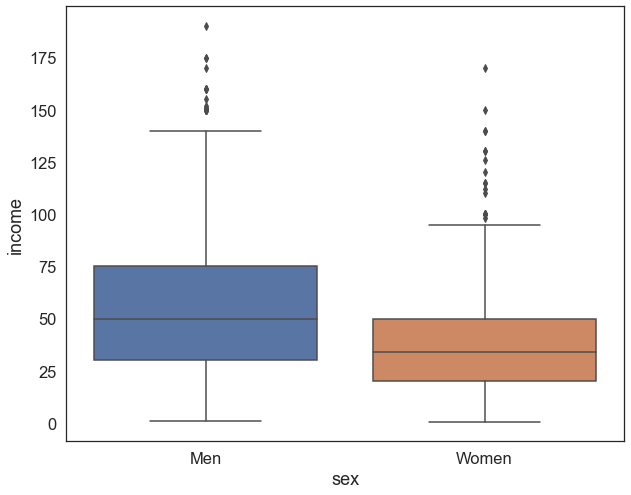
\includegraphics{notebooks/W03. Spatial Data_files/figure-pdf/cell-9-output-2.png}

}

\end{figure}

Pretty cool! We can clearly see some spikes in AQI that correspond
directly to when the state of emergency was declared. Our data is
matching expectations about reality: even though there's no information
about the state of emergency or the wildfires in our dataframe
(remember, it's just a bunch of air quality readings from sensors), we
observe a relationship between our variables (presence of wildfires and
air quality) that conforms to our expectations.

\hypertarget{exercise-4}{%
\subsection{Exercise}\label{exercise-4}}

Now, repeat the above plot but aggregate the dataframe by month rather
than by day. Store the monthly data as a new dataframe called
``monthly''.

\hypertarget{geographic-disparities}{%
\subsection{Geographic Disparities}\label{geographic-disparities}}

OK. We've got a good sense of how the wildfires affected air quality
readings across the whole state. But California is huge; there are
probably geographic disparities in how bad air quality was as a result
of the fires. Let's see which counties were worst affected by the
wildfires.

In our original dataframe, each row was a reading from a given sensor on
a given day. We grouped this data by day to create a dataframe that took
the average of \emph{all} sensors in california for each day as follows:

\texttt{df.groupby(\textquotesingle{}Day\textquotesingle{}){[}\textquotesingle{}AQI\textquotesingle{}{]}.mean()}

Now, we want to plot the average daily air quality by county; this will
involve aggregating both by day \emph{and by county}. Intuitively, we
can accomplish this changing
\texttt{\textquotesingle{}Day\textquotesingle{}} to
\texttt{{[}\textquotesingle{}Day\textquotesingle{},\textquotesingle{}COUNTY\textquotesingle{}{]}},
like so:

\texttt{df.groupby({[}\textquotesingle{}Day\textquotesingle{},\textquotesingle{}COUNTY\textquotesingle{}{]}){[}\textquotesingle{}AQI\textquotesingle{}{]}.mean()}

Let's store this new dataframe and call it ``county\_daily'':

\begin{Shaded}
\begin{Highlighting}[]
\NormalTok{county\_daily}\OperatorTok{=}\NormalTok{df.groupby([}\StringTok{\textquotesingle{}Day\textquotesingle{}}\NormalTok{,}\StringTok{\textquotesingle{}COUNTY\textquotesingle{}}\NormalTok{,])[}\StringTok{\textquotesingle{}AQI\textquotesingle{}}\NormalTok{].mean().reset\_index()}
\NormalTok{county\_daily}
\end{Highlighting}
\end{Shaded}

\begin{longtable}[]{@{}llll@{}}
\toprule\noalign{}
& Day & COUNTY & AQI \\
\midrule\noalign{}
\endhead
\bottomrule\noalign{}
\endlastfoot
0 & 1 & Alameda & 44.500000 \\
1 & 1 & Butte & 66.666667 \\
2 & 1 & Calaveras & 63.000000 \\
3 & 1 & Colusa & 78.000000 \\
4 & 1 & Contra Costa & 46.000000 \\
... & ... & ... & ... \\
17314 & 366 & Tehama & 52.000000 \\
17315 & 366 & Trinity & 36.000000 \\
17316 & 366 & Tulare & 62.666667 \\
17317 & 366 & Ventura & 23.666667 \\
17318 & 366 & Yolo & 35.000000 \\
\end{longtable}

\hypertarget{exercise-5}{%
\section{Exercise}\label{exercise-5}}

Using the \texttt{groupby} function, create a new dataframe called
``counties'' in which each row is a county, and each value is the
\textbf{maximum} AQI value in that county during the entire year. Then,
sort this dataframe in descending order using
\texttt{.sort\_values(ascending=False)}

Which county had the highest maximum AQI value? Which county had the
lowest? store the names of these counties as varables called ``highest''
and ``lowest'', shown below:

\begin{Shaded}
\begin{Highlighting}[]
\NormalTok{highest}\OperatorTok{=}\StringTok{\textquotesingle{}\textquotesingle{}}
\NormalTok{lowest}\OperatorTok{=}\StringTok{\textquotesingle{}\textquotesingle{}}

\CommentTok{\# Filter the county{-}level daily AQI readings for the worst{-}affected county}
\NormalTok{worst\_county}\OperatorTok{=}\NormalTok{county\_daily[county\_daily[}\StringTok{\textquotesingle{}COUNTY\textquotesingle{}}\NormalTok{]}\OperatorTok{==}\NormalTok{highest]}

\CommentTok{\# Filter the county{-}level daily AQI readings for the least{-}affected county}
\NormalTok{best\_county}\OperatorTok{=}\NormalTok{county\_daily[county\_daily[}\StringTok{\textquotesingle{}COUNTY\textquotesingle{}}\NormalTok{]}\OperatorTok{==}\NormalTok{lowest]}
\end{Highlighting}
\end{Shaded}

Using those two variables, lets plot the AQI values for each of these
counties individually:

\begin{Shaded}
\begin{Highlighting}[]
\CommentTok{\# plot the data from the worst affected county}
\NormalTok{plt.plot(worst\_county[}\StringTok{\textquotesingle{}Day\textquotesingle{}}\NormalTok{], worst\_county[}\StringTok{\textquotesingle{}AQI\textquotesingle{}}\NormalTok{], label}\OperatorTok{=}\NormalTok{highest)}

\CommentTok{\# plot the data from the least affected county}
\NormalTok{plt.plot(best\_county[}\StringTok{\textquotesingle{}Day\textquotesingle{}}\NormalTok{], best\_county[}\StringTok{\textquotesingle{}AQI\textquotesingle{}}\NormalTok{], label}\OperatorTok{=}\NormalTok{lowest)}

\CommentTok{\#add title and axis labels}
\NormalTok{plt.title(}\StringTok{\textquotesingle{}Daily Air Quality Index readings in California, 2020\textquotesingle{}}\NormalTok{)}
\NormalTok{plt.ylabel(}\StringTok{\textquotesingle{}AQI\textquotesingle{}}\NormalTok{)}
\NormalTok{plt.xlabel(}\StringTok{\textquotesingle{}Day of Year\textquotesingle{}}\NormalTok{)}

\CommentTok{\# add a dashed black line on August 18th (the 231st day of the year)}
\NormalTok{plt.axvline(}\DecValTok{231}\NormalTok{, color}\OperatorTok{=}\StringTok{\textquotesingle{}black\textquotesingle{}}\NormalTok{, linestyle}\OperatorTok{=}\StringTok{\textquotesingle{}{-}{-}\textquotesingle{}}\NormalTok{, label}\OperatorTok{=}\StringTok{\textquotesingle{}State of Emergency\textquotesingle{}}\NormalTok{)}
\NormalTok{plt.legend()}
\end{Highlighting}
\end{Shaded}

\begin{verbatim}
<matplotlib.legend.Legend at 0x142444c40>
\end{verbatim}

\begin{figure}[H]

{\centering 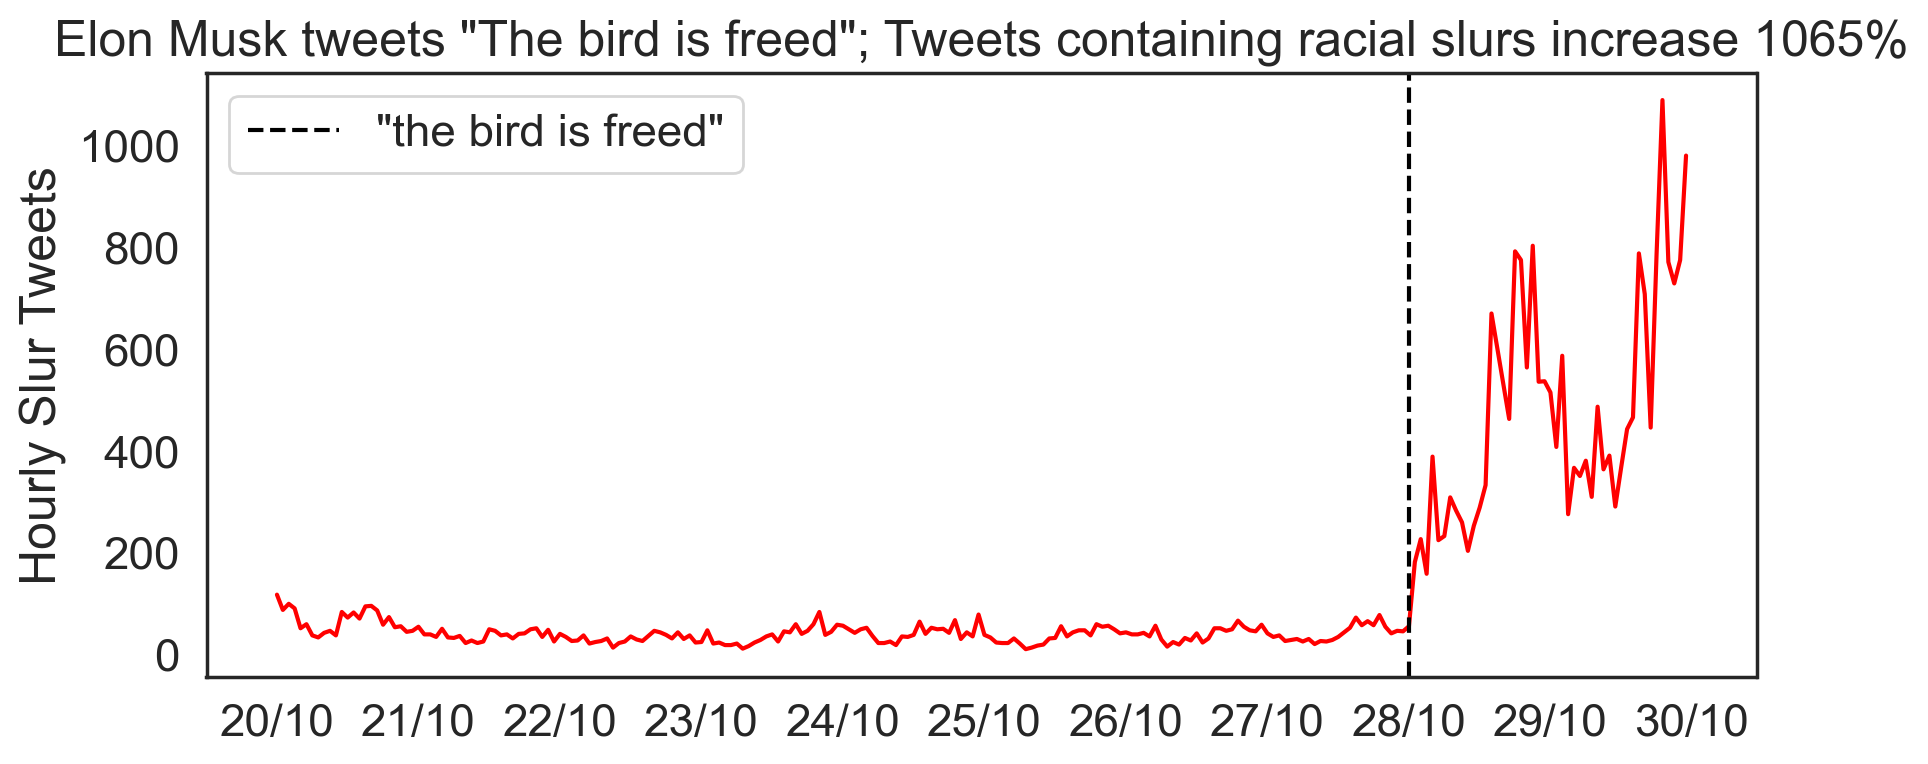
\includegraphics{notebooks/W03. Spatial Data_files/figure-pdf/cell-14-output-2.png}

}

\end{figure}

We can see that the worst affected county suffered a massive spike in
AQI following the wildfires, while the least affected county experienced
a much smaller increase in AQI.

\hypertarget{bringing-in-geography}{%
\section{Bringing in Geography}\label{bringing-in-geography}}

We can explore some limited geographic variation using the ``COUNTY''
column in our dataframe. But we actually have the latitude and longitude
of each individual sensor. We can visualize latitude and longitude data
quite simply as a scatterplot.

Remember, in our original dataframe each row is a reading from a given
sensor on a given day. The sensor's location does not vary over time, so
if we simply plot our original dataframe, we'll have loads of points on
top of each other. Let's pick a specific date, take a slice of our
dataframe on that one date, and plot it. I've picked September 9th based
on the plots above (looks like air quality was really bad).

\begin{Shaded}
\begin{Highlighting}[]
\CommentTok{\# create a variable with the date of interest, September 9th 2020. }
\NormalTok{date}\OperatorTok{=}\StringTok{\textquotesingle{}09{-}09{-}2020\textquotesingle{}}

\CommentTok{\# filter the original dataframe using this date}
\NormalTok{one\_day}\OperatorTok{=}\NormalTok{df[df[}\StringTok{\textquotesingle{}Date\textquotesingle{}}\NormalTok{]}\OperatorTok{==}\NormalTok{date]}

\CommentTok{\# create a scatterplot of sensor locations using latitude and longitude }
\NormalTok{plt.scatter(}
\NormalTok{    x}\OperatorTok{=}\NormalTok{one\_day[}\StringTok{\textquotesingle{}longitude\textquotesingle{}}\NormalTok{],}
\NormalTok{    y}\OperatorTok{=}\NormalTok{one\_day[}\StringTok{\textquotesingle{}latitude\textquotesingle{}}\NormalTok{])}

\CommentTok{\# as always, label our axes and the plot!}
\NormalTok{plt.xlabel(}\StringTok{"Longitude"}\NormalTok{)}
\NormalTok{plt.ylabel(}\StringTok{"Latitude"}\NormalTok{)}
\NormalTok{plt.title(}\StringTok{"Geographic Distribution of AQI sensors in California"}\NormalTok{)}
\end{Highlighting}
\end{Shaded}

\begin{verbatim}
Text(0.5, 1.0, 'Geographic Distribution of AQI sensors in California')
\end{verbatim}

\begin{figure}[H]

{\centering 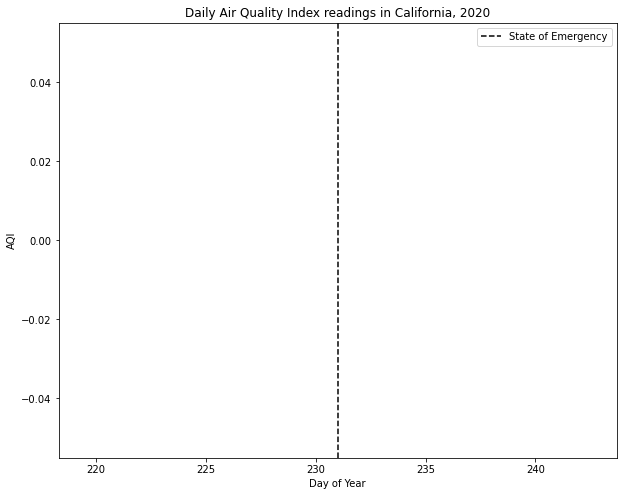
\includegraphics{notebooks/W03. Spatial Data_files/figure-pdf/cell-15-output-2.png}

}

\end{figure}

If you close your eyes and imagine the shape of California, you can
probably see its outline roughly traced in the points above. This plot
leaves a number of things to be desired.

\hypertarget{basemaps}{%
\subsection{Basemaps}\label{basemaps}}

First, we may want to add in a base map of some kind so we can have a
better sense of where each sensor is. For this, we have to import an
extra library called ``Basemap''

\begin{Shaded}
\begin{Highlighting}[]
\CommentTok{\# import Basemap library}
\ImportTok{from}\NormalTok{ mpl\_toolkits.basemap }\ImportTok{import}\NormalTok{ Basemap}

\CommentTok{\# create a basemap, call it \textquotesingle{}map\textquotesingle{}}
\BuiltInTok{map} \OperatorTok{=}\NormalTok{ Basemap(projection}\OperatorTok{=}\StringTok{\textquotesingle{}lcc\textquotesingle{}}\NormalTok{, resolution}\OperatorTok{=}\StringTok{\textquotesingle{}l\textquotesingle{}}\NormalTok{, }\CommentTok{\# this selects the projection of the map.}
\NormalTok{            lat\_0}\OperatorTok{=}\FloatTok{37.5}\NormalTok{, lon\_0}\OperatorTok{={-}}\DecValTok{119}\NormalTok{, }\CommentTok{\# this sets the center of the map }
\NormalTok{            width}\OperatorTok{=}\FloatTok{1E6}\NormalTok{, height}\OperatorTok{=}\FloatTok{1.2E6}\NormalTok{) }\CommentTok{\# this sets the window that we\textquotesingle{}re looking at, in meters.}

\CommentTok{\# We can add features to our blank basemap, including coastlines, as well as state and country boundaries. }
\BuiltInTok{map}\NormalTok{.drawcoastlines(color}\OperatorTok{=}\StringTok{\textquotesingle{}black\textquotesingle{}}\NormalTok{)}
\BuiltInTok{map}\NormalTok{.drawcountries(color}\OperatorTok{=}\StringTok{\textquotesingle{}black\textquotesingle{}}\NormalTok{)}
\BuiltInTok{map}\NormalTok{.drawstates(color}\OperatorTok{=}\StringTok{\textquotesingle{}gray\textquotesingle{}}\NormalTok{)}

\CommentTok{\# Finally, we add in our AQI sensor data on top of the basemap.}
\BuiltInTok{map}\NormalTok{.scatter(}
\NormalTok{    one\_day[}\StringTok{\textquotesingle{}longitude\textquotesingle{}}\NormalTok{], }
\NormalTok{    one\_day[}\StringTok{\textquotesingle{}latitude\textquotesingle{}}\NormalTok{], }
\NormalTok{    latlon}\OperatorTok{=}\VariableTok{True}\NormalTok{)}

\CommentTok{\# as always, title your figure}
\NormalTok{plt.title(}\StringTok{"Geographic Distribution of AQI sensors in California"}\NormalTok{)}
\end{Highlighting}
\end{Shaded}

\begin{verbatim}
ImportError: dlopen(/Users/ollieballinger/miniconda3/envs/geo/lib/python3.9/site-packages/_geoslib.cpython-39-darwin.so, 0x0002): tried: '/Users/ollieballinger/miniconda3/envs/geo/lib/python3.9/site-packages/_geoslib.cpython-39-darwin.so' (mach-o file, but is an incompatible architecture (have 'x86_64', need 'arm64')), '/System/Volumes/Preboot/Cryptexes/OS/Users/ollieballinger/miniconda3/envs/geo/lib/python3.9/site-packages/_geoslib.cpython-39-darwin.so' (no such file), '/Users/ollieballinger/miniconda3/envs/geo/lib/python3.9/site-packages/_geoslib.cpython-39-darwin.so' (mach-o file, but is an incompatible architecture (have 'x86_64', need 'arm64'))
\end{verbatim}

That's looking a bit better! We now have a much better sense of the
actual distribution of these sensors within california. People who know
the area will recognize clusters of sensors around San Francisco and Los
Angeles; This makes sense, given that these areas have a higher
population density. However, our plot is still missing some pretty
important information: the actual AQI readings!

\hypertarget{colormaps}{%
\subsection{Colormaps}\label{colormaps}}

The whole point of plotting these sensors is to understand the spatial
distribution of air pollution from the 2020 wildfires.

The EPA published the following
\href{https://www.airnow.gov/aqi/aqi-basics/}{table} on their website,
which creates a color-coded scale of AQI values that corresponds to the
impact thereof on human health.

\begin{itemize}
\tightlist
\item
  AQI under 50 is colored green, and indicates ``Good'' air quality.
\item
  AQI between 100 and 200 is generally unhealthy
\item
  AQI over 300 is deemed hazardous.
\end{itemize}

With this in mind, quickly scroll back up to the AQI plots over time. If
you did everything correctly, you should notice that the \emph{average}
AQI value across all sensors in the worst affected county was over 600!

We'll be using the table from the EPA website to build our own color
map. In the code below, I scrape the table and turn it into a
``colormap'' (basically, a dictionary that associates numbers with
colors) that we'll use to color the AQI sensors later.

\begin{Shaded}
\begin{Highlighting}[]
\CommentTok{\# scrape the table of AQI values and corresponding colors }
\CommentTok{\# save it as a dataframe called colors}
\NormalTok{colors}\OperatorTok{=}\NormalTok{pd.read\_html(}\StringTok{\textquotesingle{}https://www.airnow.gov/aqi/aqi{-}basics/\textquotesingle{}}\NormalTok{)[}\DecValTok{0}\NormalTok{]}

\CommentTok{\# create a numerical column for AQI values by splitting the test in the "values of index" column. }
\CommentTok{\# pull out the first string, and convert it to integer}
\NormalTok{colors[}\StringTok{\textquotesingle{}aqi\textquotesingle{}}\NormalTok{]}\OperatorTok{=}\NormalTok{colors[}\StringTok{\textquotesingle{}Values of Index\textquotesingle{}}\NormalTok{].}\BuiltInTok{str}\NormalTok{.split(}\StringTok{\textquotesingle{} \textquotesingle{}}\NormalTok{).}\BuiltInTok{str}\NormalTok{[}\DecValTok{0}\NormalTok{].astype(}\BuiltInTok{int}\NormalTok{)}

\CommentTok{\# print three columns from the dataframe }
\BuiltInTok{print}\NormalTok{(colors[[}\StringTok{\textquotesingle{}aqi\textquotesingle{}}\NormalTok{,}\StringTok{\textquotesingle{}Daily AQI Color\textquotesingle{}}\NormalTok{,}\StringTok{\textquotesingle{}Levels of Concern\textquotesingle{}}\NormalTok{]])}

\CommentTok{\# create a "colormap" from this dataframe using the "Daily AQI Color" column, and the "aqi" column }
\NormalTok{aqi\_colors}\OperatorTok{=}\NormalTok{matplotlib.colors.LinearSegmentedColormap.from\_list(colors[}\StringTok{\textquotesingle{}aqi\textquotesingle{}}\NormalTok{],colors[}\StringTok{\textquotesingle{}Daily AQI Color\textquotesingle{}}\NormalTok{])}
\end{Highlighting}
\end{Shaded}

\begin{verbatim}
   aqi Daily AQI Color               Levels of Concern
0    0           Green                            Good
1   51          Yellow                        Moderate
2  101          Orange  Unhealthy for Sensitive Groups
3  151             Red                       Unhealthy
4  201          Purple                  Very Unhealthy
5  301          Maroon                       Hazardous
\end{verbatim}

Now, we can use this ``aqi\_colors'' object as a color palette later
when we plot the AQI sensors. This way, we will know that green and
yellow points are OK, while red and purple points represent hazardous
levels of air pollution. I've annotated the code above, but it's ok if
you don't get all of it. You could simply load a different colormap in
one line of code; check out the documentation
\href{https://matplotlib.org/stable/tutorials/colors/colormaps.html}{here}.

\begin{Shaded}
\begin{Highlighting}[]
\BuiltInTok{map} \OperatorTok{=}\NormalTok{ Basemap(projection}\OperatorTok{=}\StringTok{\textquotesingle{}lcc\textquotesingle{}}\NormalTok{, resolution}\OperatorTok{=}\StringTok{\textquotesingle{}l\textquotesingle{}}\NormalTok{, }
\NormalTok{            lat\_0}\OperatorTok{=}\FloatTok{37.5}\NormalTok{, lon\_0}\OperatorTok{={-}}\DecValTok{119}\NormalTok{,}
\NormalTok{            width}\OperatorTok{=}\FloatTok{1E6}\NormalTok{, height}\OperatorTok{=}\FloatTok{1.2E6}\NormalTok{)}

\BuiltInTok{map}\NormalTok{.drawcoastlines(color}\OperatorTok{=}\StringTok{\textquotesingle{}black\textquotesingle{}}\NormalTok{)}
\BuiltInTok{map}\NormalTok{.drawcountries(color}\OperatorTok{=}\StringTok{\textquotesingle{}black\textquotesingle{}}\NormalTok{)}
\BuiltInTok{map}\NormalTok{.drawstates(color}\OperatorTok{=}\StringTok{\textquotesingle{}gray\textquotesingle{}}\NormalTok{)}

\BuiltInTok{map}\NormalTok{.scatter(}
\NormalTok{      one\_day[}\StringTok{\textquotesingle{}longitude\textquotesingle{}}\NormalTok{], }
\NormalTok{      one\_day[}\StringTok{\textquotesingle{}latitude\textquotesingle{}}\NormalTok{], }
\NormalTok{      latlon}\OperatorTok{=}\VariableTok{True}\NormalTok{, }
\NormalTok{      c}\OperatorTok{=}\NormalTok{one\_day[}\StringTok{\textquotesingle{}AQI\textquotesingle{}}\NormalTok{], }\CommentTok{\# We\textquotesingle{}re adding that }
\NormalTok{      cmap}\OperatorTok{=}\NormalTok{aqi\_colors, }
\NormalTok{      vmin}\OperatorTok{=}\DecValTok{0}\NormalTok{, }
\NormalTok{      vmax}\OperatorTok{=}\DecValTok{300}\NormalTok{)}


\NormalTok{plt.title(}\StringTok{\textquotesingle{}Air Quality on September 9th, 2020\textquotesingle{}}\NormalTok{)}
\NormalTok{plt.colorbar(label}\OperatorTok{=}\StringTok{\textquotesingle{}Air Quality Index\textquotesingle{}}\NormalTok{)}\OperatorTok{;}
\end{Highlighting}
\end{Shaded}

\begin{figure}[H]

{\centering 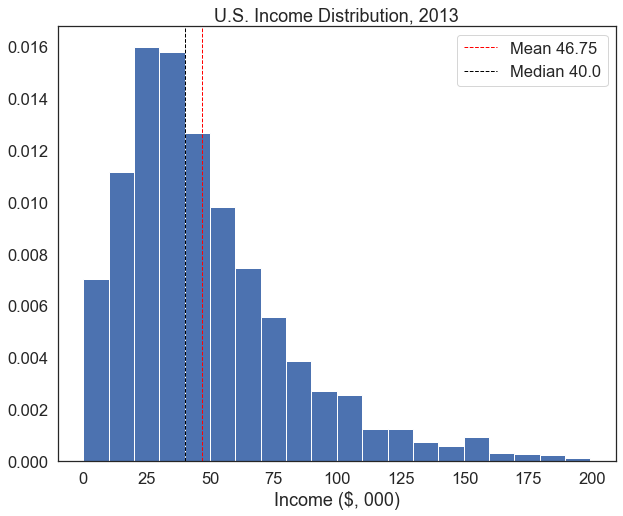
\includegraphics{notebooks/W03. Spatial Data_files/figure-pdf/cell-18-output-1.png}

}

\end{figure}

This plot gives us a good sense of which areas were worst affected by
the wildfires on September 9th, 2020. Areas in the central valley
suffered particularly bad air quality, with AQI reaching hazardous
levels in some areas.

\hypertarget{exercise-6}{%
\subsection{Exercise}\label{exercise-6}}

So far, we've been plotting data from one day, using a dataframe we
generated by filtering the date column like so:
\texttt{one\_day=df{[}df{[}\textquotesingle{}Date\textquotesingle{}{]}==\textquotesingle{}09-09-2020\textquotesingle{}{]}}
(date format is day-month-year).

Using the code from the previous cell, generate a plot of AQI on March
2nd, 2020. After that, use the groupby function to generate a plot of
the maximum AQI reading for each sensor and plot it.

If you've followed along this far, well done! we've come a long way from
a spreadsheet full of sensor readings. But we can go even further!

\hypertarget{advanced-satellite-imagery-and-interactivity}{%
\section{Advanced: Satellite Imagery and
Interactivity}\label{advanced-satellite-imagery-and-interactivity}}

The AQI plots we've generated above give us a good sense of where the
worst air pollution was on a given day; but we're still basically
\emph{inferring} the presence of fires. Luckily, we don't have to do
that. The plumes of smoke generated by the fires were so vast that they
were visible from space. There are a variety of satellites that image
the earth each day (some, like GOES-17, take a picture every few
minutes!).

NASA's Moderate Resolution Imaging Spectroradiometer (MODIS) satellites
take a picture of the same spot on earth nearly every day. So far, we've
been looking at September 9th as a particularly bad day for air quality
in California. Let's have a look at a satellite image from that day. A
Python library called ipyleaflet contains some useful functions that let
us pull up an interactive map of satellite imagery.

\begin{Shaded}
\begin{Highlighting}[]
\CommentTok{\# import the map making modules from ipyleaflet}
\ImportTok{from}\NormalTok{ ipyleaflet }\ImportTok{import}\NormalTok{ Map, Marker, basemaps, basemap\_to\_tiles,Circle}
\ImportTok{from}\NormalTok{ ipywidgets }\ImportTok{import}\NormalTok{ HTML}

\CommentTok{\# let create an interactive Map object called "satellite\_map"}
\NormalTok{satellite\_map }\OperatorTok{=}\NormalTok{ Map(}
\NormalTok{  basemap}\OperatorTok{=}\NormalTok{basemap\_to\_tiles( }\CommentTok{\#this function lets us pick from a list of basemaps for our interactive map}
\NormalTok{    basemaps.NASAGIBS.ModisTerraTrueColorCR, }\StringTok{"2020{-}09{-}09"} \CommentTok{\# here we\textquotesingle{}re specifying that we want MODIS imagery, and the date that we want it from  }
\NormalTok{  ),}
\NormalTok{  center}\OperatorTok{=}\NormalTok{(}\FloatTok{36.77}\NormalTok{, }\OperatorTok{{-}}\FloatTok{119.41}\NormalTok{), }\CommentTok{\# then, we want to center the map on california. these coordinates do that}
\NormalTok{  zoom}\OperatorTok{=}\DecValTok{5}\NormalTok{, }\CommentTok{\#finally, we want to set the zoom level of the map. }
\NormalTok{)}

\CommentTok{\# once we\textquotesingle{}ve created the map object we can make it bigger or smaller. let\textquotesingle{}s make it 700 pixels tall. }
\NormalTok{satellite\_map.layout.height }\OperatorTok{=} \StringTok{\textquotesingle{}700px\textquotesingle{}}

\CommentTok{\# now, we visualize it.}
\NormalTok{satellite\_map}
\end{Highlighting}
\end{Shaded}

\begin{verbatim}
Map(center=[36.77, -119.41], controls=(ZoomControl(options=['position', 'zoom_in_text', 'zoom_in_title', 'zoom…
\end{verbatim}

This is a pretty striking image of the West Coast of the U.S. We can see
fluffy white clouds to the East and West, but in the center of the map
plumes of brown smoke emanate from wildfires in California and Oregon.
Use the + - keys in the top left to zoom in, see if you can spot some
wildfires.

\hypertarget{exercise-7}{%
\subsection{Exercise}\label{exercise-7}}

Try changing the code in the cell above to display an image from
September 15th. You could even try importing a different basemap (like
nighttime lights) using this
\href{https://ipyleaflet.readthedocs.io/en/latest/map_and_basemaps/basemaps.html}{list
of basemaps}.

\hypertarget{combining-sensors-and-satellite-images}{%
\section{Combining sensors and satellite
images}\label{combining-sensors-and-satellite-images}}

A cool part of working with spatial data is that we can combine two
completeley different datasets using spatial information. We can add the
AQI sensor data as points to this map.

\begin{Shaded}
\begin{Highlighting}[]
\CommentTok{\# grab the first row from our September 9th dataframe}
\NormalTok{row}\OperatorTok{=}\NormalTok{one\_day.iloc[}\DecValTok{0}\NormalTok{]}
\BuiltInTok{print}\NormalTok{(row)}

\CommentTok{\# This part uses the AQI value in this row (72), and looks up the corresponding color in the colormap we created earlier }
\NormalTok{color}\OperatorTok{=}\NormalTok{matplotlib.colors.rgb2hex(aqi\_colors(row[}\StringTok{\textquotesingle{}AQI\textquotesingle{}}\NormalTok{]))}

\CommentTok{\# Now we create a Circle object using the latitude and longitude from the row, and color it using the color we just selected}
\NormalTok{point}\OperatorTok{=}\NormalTok{Circle(location}\OperatorTok{=}\NormalTok{(row[}\StringTok{\textquotesingle{}latitude\textquotesingle{}}\NormalTok{],row[}\StringTok{\textquotesingle{}longitude\textquotesingle{}}\NormalTok{]), color}\OperatorTok{=}\NormalTok{color)}

\CommentTok{\# Add this as a layer to the satellite\_map object}
\NormalTok{satellite\_map.add\_layer(point)}

\CommentTok{\# Display the updated map}
\NormalTok{satellite\_map}
\end{Highlighting}
\end{Shaded}

\begin{verbatim}
Date                       2020-09-09 00:00:00
Site ID                               60010007
POC                                          3
PM                                        22.3
AQI                                         72
Site Name                            Livermore
CBSA_NAME    San Francisco-Oakland-Hayward, CA
COUNTY                                 Alameda
latitude                             37.687526
longitude                          -121.784217
Month                                        9
Day                                        253
Name: 249, dtype: object
\end{verbatim}

\begin{verbatim}
Map(center=[36.77, -119.41], controls=(ZoomControl(options=['position', 'zoom_in_text', 'zoom_in_title', 'zoom…
\end{verbatim}

It's a bit hard to see, but we've plotted an AQI sensor! its under the
cloud of smoke in the center of the map. You can zoom in to get a closer
look. looks like AQI was pretty bad at this location.

Having plotted one point, we can now plot all the points on September
9th! to do so, we can use the \texttt{iterrows} function in Pandas
which, suprisingly, lets you iterate over rows in a dataframe. The first
line of code below allows us to iterate over the rows in the
\texttt{one\_day} dataframe. It will then run everything in the indented
block for each row; in other words, for each row, it will:

\begin{enumerate}
\def\labelenumi{\arabic{enumi}.}
\tightlist
\item
  use the row's value in the AQI value to select a color for the point
\item
  create a point object using the latitude and longitude columns
\item
  add that point to the satellite map.
\end{enumerate}

\begin{Shaded}
\begin{Highlighting}[]
\ControlFlowTok{for}\NormalTok{ index, row }\KeywordTok{in}\NormalTok{ one\_day.iterrows():}
\NormalTok{  color}\OperatorTok{=}\NormalTok{matplotlib.colors.rgb2hex(aqi\_colors(row[}\StringTok{\textquotesingle{}AQI\textquotesingle{}}\NormalTok{]))}
\NormalTok{  point}\OperatorTok{=}\NormalTok{Circle(location}\OperatorTok{=}\NormalTok{(row[}\StringTok{\textquotesingle{}latitude\textquotesingle{}}\NormalTok{],row[}\StringTok{\textquotesingle{}longitude\textquotesingle{}}\NormalTok{]), color}\OperatorTok{=}\NormalTok{color)}
\NormalTok{  satellite\_map.add\_layer(point)}

\CommentTok{\# display the map}
\NormalTok{satellite\_map}
\end{Highlighting}
\end{Shaded}

\begin{verbatim}
Map(center=[36.77, -119.41], controls=(ZoomControl(options=['position', 'zoom_in_text', 'zoom_in_title', 'zoom…
\end{verbatim}

Theres a pretty striking trend in this data. If you zoom in, you'll see
that the AQI sensors to the East are all green since they are up-wind
from the fires. A few kilometers downwind of the fires, the AQI sensors
display very high readings. Remember, our AQI data and the satellite
imagery are derived from totally different sources, and are totally
different types of data, but they seem to be telling us the same story.
They actually complement each other in important ways. In our original
plot of the AQI sensors without satellite imagery, we could tell that
there was bad air quality on September 9th, but some sensors were green
and others were red. The satellite image shows us that the variation in
AQI across California on September 9th was due to the direction of the
wind, blowing the smoke from the wildfires westward.

\hypertarget{extension-1}{%
\section{Extension}\label{extension-1}}

Now, to save some hassle we can package all the code we used to generate
this map into one clean function. Because we're effectively just
changing the date, we can configure this function so that we can feed it
a different date, and it will grab a satellite image and filter our
dataframe for values occuring on that day. Then, we can draw a new map
in one line of code.

\begin{Shaded}
\begin{Highlighting}[]
\KeywordTok{def}\NormalTok{ satellite\_plot(date):}
  
\NormalTok{  ymd}\OperatorTok{=}\NormalTok{datetime.strptime(date, }\StringTok{\textquotesingle{}}\SpecialCharTok{\%d}\StringTok{{-}\%m{-}\%Y\textquotesingle{}}\NormalTok{).strftime(}\StringTok{\textquotesingle{}\%Y{-}\%m{-}}\SpecialCharTok{\%d}\StringTok{\textquotesingle{}}\NormalTok{)}

\NormalTok{  satellite\_map }\OperatorTok{=}\NormalTok{ Map(}
\NormalTok{    basemap}\OperatorTok{=}\NormalTok{basemap\_to\_tiles(}
\NormalTok{      basemaps.NASAGIBS.ModisTerraTrueColorCR, ymd}
\NormalTok{    ),}
\NormalTok{    center}\OperatorTok{=}\NormalTok{(}\FloatTok{36.77}\NormalTok{, }\OperatorTok{{-}}\FloatTok{119.41}\NormalTok{),}
\NormalTok{    zoom}\OperatorTok{=}\DecValTok{6}\NormalTok{,}
\NormalTok{  )}

\NormalTok{  satellite\_map.layout.height }\OperatorTok{=} \StringTok{\textquotesingle{}700px\textquotesingle{}}

\NormalTok{  one\_day}\OperatorTok{=}\NormalTok{df[df[}\StringTok{\textquotesingle{}Date\textquotesingle{}}\NormalTok{]}\OperatorTok{==}\NormalTok{date]}

  \ControlFlowTok{for}\NormalTok{ index, row }\KeywordTok{in}\NormalTok{ one\_day.iterrows():}
\NormalTok{    color}\OperatorTok{=}\NormalTok{matplotlib.colors.rgb2hex(aqi\_colors(row[}\StringTok{\textquotesingle{}AQI\textquotesingle{}}\NormalTok{]))}
\NormalTok{    point}\OperatorTok{=}\NormalTok{Circle(location}\OperatorTok{=}\NormalTok{(row[}\StringTok{\textquotesingle{}latitude\textquotesingle{}}\NormalTok{],row[}\StringTok{\textquotesingle{}longitude\textquotesingle{}}\NormalTok{]), color}\OperatorTok{=}\NormalTok{color)}
\NormalTok{    point.popup }\OperatorTok{=}\NormalTok{ HTML(}\BuiltInTok{str}\NormalTok{(row[}\StringTok{\textquotesingle{}Site Name\textquotesingle{}}\NormalTok{]))    }
\NormalTok{    satellite\_map.add\_layer(point)}
  \ControlFlowTok{return}\NormalTok{ satellite\_map}
\end{Highlighting}
\end{Shaded}

Now, we can simply change the date in the function and view both
satellite imagery and AQI sensor data from a given day. Look at this
clear day from February 3rd.

\begin{Shaded}
\begin{Highlighting}[]
\NormalTok{satellite\_plot(}\StringTok{\textquotesingle{}02{-}03{-}2020\textquotesingle{}}\NormalTok{)}
\end{Highlighting}
\end{Shaded}

\begin{verbatim}
Map(center=[36.77, -119.41], controls=(ZoomControl(options=['position', 'zoom_in_text', 'zoom_in_title', 'zoom…
\end{verbatim}

All the AQI sensors are showing green values, indicating generally good
air quality. The satellite image shows a few wispy clouds, but no thick
yellow smoke. Now change the date to September 15th, and see what
happens!



\end{document}
